\documentclass[8pt]{beamer}
\usepackage{graphicx}
\usepackage{booktabs} % For professional looking tables
\usepackage{threeparttable} % For table notes
\usepackage{multirow} % For cells that span multiple rows
\usepackage{glossaries} % In case you use \gls{} in the table
\usepackage{algorithm}
\usepackage{algpseudocode}
\usepackage{amsmath}
\usepackage[backend=biber,style=authoryear]{biblatex}
\addbibresource{../bibliography/mybib}
\usepackage{comment}

% Define glossary entries if not already defined
\newglossaryentry{fp}{name={FP}, description={Floating Point}}

\newcommand{\backupbegin}{
	\newcounter{framenumberappendix}
	\setcounter{framenumberappendix}{\value{framenumber}}
}
\newcommand{\backupend}{
	\addtocounter{framenumberappendix}{-\value{framenumber}}
	\addtocounter{framenumber}{\value{framenumberappendix}} 
}

\mode<presentation> {
	\usetheme{CambridgeUS}
	\usecolortheme{dolphin}
	
	% Remove the navigation symbols
	\setbeamertemplate{navigation symbols}{}
	
	% Explicitly set the headline to be empty
	\setbeamertemplate{headline}{}
	
	% Customize footline to include section and page number
	\setbeamertemplate{footline}{%
		\leavevmode%
		\hbox{%
			\begin{beamercolorbox}[wd=.5\paperwidth,ht=2.25ex,dp=1ex,left]{section in head/foot}%
				\usebeamerfont{section in head/foot}\hspace*{2ex}\insertsection
			\end{beamercolorbox}%
			\begin{beamercolorbox}[wd=.5\paperwidth,ht=2.25ex,dp=1ex,right]{section in head/foot}%
				\usebeamerfont{section in head/foot}\insertframenumber{} / \inserttotalframenumber\hspace*{2ex}
			\end{beamercolorbox}%
		}%
		\vskip0pt%
	}
}




\title[PhD Defense - Yarib Nevarez]{Low-Power Neural Network Accelerators:
	\\Advancements in Custom Floating-Point Techniques}
\author{Yarib Nevarez}
\institute{Universität Bremen}
\date{May 22, 2024}

\begin{document}
	
	\begin{titlepage} % Suppresses displaying the page number on the title page and the subsequent page counts as page 1
	\singlespacing
	%	\raggedleft % Right align the title page
	
	\rule{1pt}{\textheight} % Vertical line
	\hspace{0.03\textwidth} % Whitespace between the vertical line and title page text
	\parbox[b]{0.9\textwidth}{ % Paragraph box for holding the title page text, adjust the width to move the title page left or right on the page
		 
		{\Large \bfseries   
			Low-Power Neural Network Accelerators:\\[2mm] %[0.1\baselineskip]
			Advancements in Custom Floating-Point Techniques\\[2mm]\\[2mm]
		}\\[2\baselineskip]
		% {\Huge \bfseries
		% Low-Power~Design\\[1mm] %[0.1\baselineskip]
		% for~High-Performance\\[1mm] %[0.1\baselineskip]
		% and~Yield-Enhanced\\[1mm] %[0.12\baselineskip]
		% 3D~Interconnects
		% }\\[2\baselineskip] 
		% 
		%Title 
		{\large\textit{\setstretch{4} Dissertation zur Erlangung des akademischen Grades \\[0.03\baselineskip]
				Doktor-Ingenieur (Dr.-Ing.) im Fach Elektrotechnik \\[0.03\baselineskip]
				und Informationstechnik}}\\[3\baselineskip] % Subtitle or further description
		{\Large\textsc{Yarib Nevarez}}\\[13\baselineskip] % Author name, lower case for consistent small caps     
		%     \vspace{0.42\textheight} 
		\bgroup
		\def\arraystretch{1.2}%  1 is the default, change whatever you need
		{\normalsize
			\begin{tabular}{l l}
				
				
				1.\ Gutachter:  & Prof.~Dr.~Alberto Garc\'ia-Ortiz\\
				2.\ Gutachter: & Prof.~Dr.~Frans Widdershoven\\
				\\ 
				Eingereicht am: & 22.05.2024 \\
				%Tag des Promotionskolloquiums: & \_\_.\_\_.2024 \\
				
			\end{tabular}
		}
		\egroup
		\vspace{0.1\textheight} % Whitespace between the title block and the publisher
		
		{\hfill 
\includegraphics[height=2.5em,keepaspectratio]{./figures/UHB_Logo_schwarz.pdf}}
	}
	
\end{titlepage}	
	
	\chapter{Introduction}\label{chap.intro}
\minitoc
\section{Preamble}
The use of \gls{ai}/\gls{ml} is entering a new era with ubiquitous connected devices to enhance intelligence, functionality, and connectivity in our increasingly digital world. However, \gls{ai}/\gls{ml} algorithms are computationally and energy intensive, this represents an important challenge for sustainability and realization. Therefore, this digital transformation requires hardware design methodologies that reconcile efficiency with inference quality, and adaptability.

Hardware acceleration for embedded devices is expected to drive further advancements in \gls{ai}/\gls{ml} technologies, paving the way for transformative applications in Edge AI, \gls{iot}, \gls{fl}, Industry 4.0, and smart cities. Interoperability of quantization approaches and model compression techniques are often favored in decentralized machine learning approaches and mission critical domains to ensure the safety and reliability of \gls{ai} systems. In this line, the development of efficient compute engines remains a crucial enabler for unlocking the full potential of \gls{ai}/\gls{ml} technologies.

This section presents the preamble to investigate design methodologies for low-power hardware accelerators of \gls{ai}/\gls{ml} algorithms focusing on inference quality, scalability, versatility, and compatibility as design philosophy.

\subsection{AI/ML in Industry 4.0}
\gls{ai} and \gls{ml} play a crucial role in the context of Industry 4.0, which is characterized by the integration of digital technologies into manufacturing and industrial processes to create a more connected, intelligent, and automated environment.

\subsubsection{Industry 4.0}
Since the beginning of industrialization, technological leaps have led to paradigm shifts, now called "industrial revolutions": from mechanization, electrification, and later, digitalization (the so-called 3rd industrial revolution). Based on the advanced digitalization within factories, the combination of Internet technologies and future-oriented technologies in the field of "smart" things (machines and products) seems to result in a new fundamental paradigm shift in industrial production. Emerging from this future expectation, the term "Industry 4.0" was established for an expected "4th industrial revolution"~\cite{lasi2014industry}.


\subsubsection{Internet-of-Things in Industry}
% Context background
To build the emerging environment of Industry 4.0, disruptive technologies are required to handle autonomous communications between all industrial embedded computers throughout the factory and the Internet. Such technologies offer the potential to transform the industry along the entire production chain and stimulate productivity and overall economic growth \cite{espinoza2020estimating}. These technologies include cloud computing, big data, and specially a new generation of \gls{iot} devices fused with \gls{cps}, safety-security, augmented reality, \gls{ml}, and hardware accelerators~\cite{alcacer2019scanning}.

\subsubsection{Artificial Intelligence in Internet-of-Things}
% Particular background
The continuous evolution of \gls{ai} algorithms and \gls{iot} devices has not only made \gls{ai} the major workload running on these embedded devices, but has transformed \gls{ai} into the main approach for industrial solutions, especially in the rise of Industry 4.0~\cite{alcacer2019scanning}. As a result, the term of \gls{iot} has also been redefined as \gls{ai} of Things (AIoT) to emphasize the impact on this technology~\cite{zhang2020empowering}.

There is a clear motivation to run \gls{ai}/\gls{ml} algorithms on \gls{iot} devices because of~\cite{loh20201}:

\begin{itemize}
	\item \textbf{Feasibility of Mission-Critical with Real-Time Processing}. Deploying \gls{ml} models directly on embedded devices, inference can be performed locally without relying on cloud or remote servers. This enables real-time decision-making and faster response times, which is critical for applications such as autonomous vehicles, industrial automation, and robotics.
	\item \textbf{Privacy and Security of Data}. Processing data locally on embedded devices helps preserve data privacy and security. Instead of transmitting sensitive data to external servers, the data stays inside the device, reducing the risk of data breaches or unauthorized access.
	\item \textbf{Offline Operation Capability and Robustness for Stressed Communication}. Embedded devices often work in environments where network connectivity may be limited or intermittent. Locally running \gls{ml} models allow the device to continue to function and make intelligent decisions even when disconnected from the network.
\end{itemize}


\subsection{Approximation in AI/ML}
Based on the error tolerance in \gls{ml} algorithms, a promising solution is approximate computing. This paradigm has been used in a wide range of applications to increase hardware efficiency~\cite{han2013approximate}. For neural network applications, two main approximation strategies are used, namely network compression and classical approximate computing~\cite{bouvier2019spiking}.

\subsubsection{Network Compression and Quantization}
Researchers focusing on embedded applications started lowering the precision of weights and activation maps to shrink the memory footprint of the large number of parameters representing \glspl{ann}, a method known as network quantization. In this manner, reduced bit precision causes a small accuracy loss~\cite{courbariaux2015binaryconnect, han2015deep, hubara2017quantized, rastegari2016xnor}. In addition to quantization, network pruning reduces the model size by removing structural portions of the parameters and its associated computations~\cite{lecun1989optimal,hassibi1992second}. This method has been identified as an effective technique to improve the efficiency of \gls{cnn} for applications with limited computational and energy  budget~\cite{molchanov2016pruning,li2016pruning, liu2018rethinking}. These techniques leverage the intrinsic error-tolerance of neural networks, as well as their ability to recover from accuracy degradation while training.

\subsubsection{Error Tolerance in AI/ML Algorithms}
An algorithm can be regarded as error-tolerant or error-resilient when it provides a result with the required accuracy while utilizing processing components with a certain degree of inaccuracy. There are several reasons why an algorithm/application is tolerant of errors as discussed in~\cite{chippa2013analysis}. These include noisy or redundant data of the algorithm, approximate or probabilistic computations within the algorithm, and a range of acceptable outcomes. This is the case of \gls{ai}/\gls{ml} models.


\subsubsection{Approximate Computing}
%Geneal background
Approximate computing is a design paradigm that is able to tradeoff computation quality (e.g., accuracy) and computational efficiency (e.g., in run-time, chip-area, and/or energy) by exploiting the error resilience of applications/algorithms~\cite{gillani2020exploiting, zhang2015approxann}. Data redundancy of neural networks incorporate a certain degree of resilience against random external and internal perturbations;
for instance, noisy inputs and random hardware errors. This property can be exploited in a cross-layer resilience approach~\cite{carter2010design}: by leveraging error tolerance at algorithmic-level, it can be allowed a certain degree of inaccuracies at the computing-level. This approach consists of designing processing elements that approximate their computation by employing cleverly modified algorithmic logic units~\cite{han2013approximate}.

Approximate computing techniques allow substantial enhancement in processing efficiency with moderated accuracy degradation. Some research papers have shown the feasibility of applying approximate computing to the inference stage of neural networks~\cite{lotrivc2012applicability, han2013approximate, du2014leveraging, mrazek2016design, sarwar2016multiplier, zervakis2021approximate}. Such techniques usually demonstrated small inference accuracy degradation, but significant enhancement in computational performance, chip-area, and energy consumption. Hence, by taking advantage of the intrinsic error-tolerance of neural networks, approximate computing is positioned as a promising approach for \gls{ai}/\gls{ml} computation on resource-limited devices.

% Problem to solve
\section{Problem Statement}
A fundamental problem for the rise of \gls{ai} in Industry 4.0 is the fact that \gls{ml} models, particularly \glspl{cnn} and \glspl{ann}, are highly computational and data intensive. This brings significant challenges across the spectrum of computing hardware, specially in the scope of embedded systems~\cite{venkataramani2016efficient}. The most deployed models and also some of the most computationally and energy expensive are for computer vision using \glspl{cnn}. Compared to the conventional image processing methods, the accuracy of \gls{cnn} has improved significantly that by 2015, a human can no longer beat a computer in image classification~\cite{loh20201}. The early development of \glspl{cnn} before 2016 mainly focused on accuracy improvement without considering computational costs. While accuracy of deep \gls{cnn} for image classification improved 24\% between 2012 and 2016, the demand on hardware resources increased more than $10\times$. Starting from 2017, significant attention was paid to improve hardware efficiency in terms of compute power, memory bandwidth, and power consumption, while maintaining accuracy at a similar level to human perception~\cite{venkataramani2016efficient}.

\subsection{Power Dissipation}
Consequently, the recent breakthroughs in \gls{ai}/\gls{ml} applications have brought significant advancements in neural network processors~\cite{jouppi2017datacenter}. To bring the inference speed to an acceptable level, \gls{asic} with \gls{npu} are becoming ubiquitous in both embedded and general purpose computing. \glspl{npu} perform several tera operations per second in a confined area, as a consequence, they become subject to elevated on-chip power densities that rapidly result in excessive on-chip temperatures during operation~\cite{amrouch2020npu}. Subsequently, the elevated power supply, physical dimensions, heat sink and air cooling requirements demand a balance between the benefits of \gls{ml} against its environmental and financial costs. This outcome is expected on parallel computing techniques, yet unsustainable for resource-constrained devices.
Therefore, radical changes to conventional computing are required in order to sustain and improve performance while satisfying energy and temperature constraints~\cite{gillani2020exploiting}.

\subsection{Aggressive Quantization}
Furthermore, reducing the compute hardware with aggressive quantization such as binary \cite{courbariaux2015binaryconnect}, ternary \cite{lin2015neural}, and mixed precision (2-bit activations and ternary weights) \cite{colangelo2018exploration} typically incur significant accuracy degradation for very low precisions, especially for complex problems~\cite{faraone2019addnet}, such as: semantic segmentation, machine translation, language generation, playing agents, image/music generation, and medical applications.

While aggressive quantization can be beneficial for resource-constrained environments and non-critical applications, careful consideration and a more conservative approach are essential for ensuring the safety and reliability of \gls{ai}/\gls{ml} systems in mission-critical domains. Quantization techniques must be chosen wisely, keeping in mind the specific requirements and constraints of each application.

\subsection{Interoperability}
Aggressive quantization might not be supported by all hardware platforms. Custom hardware accelerators may have limitations on the precision they can handle effectively, limiting the compatibility and portability of aggressively quantized models. Aggressively quantized models may not be compatible with all frameworks, libraries, or \gls{ai} platforms, limiting their interoperability and portability across different environments. In real-world deployment scenarios, there may be constraints and requirements that make aggressive quantization impractical, especially when high accuracy, compatibility, portability, and interoperability are necessary.
%%%%%%%%%%%%%%
\section{Working Hypothesis}
% Alternatives and possible solutions for the problem
Despite its benefits, quantization may lead to a trade-off between model accuracy and hardware efficiency. Aggressive quantization can cause a loss of model accuracy due to information loss from reduced precision. Therefore, finding the right balance between quantization levels and model accuracy becomes a critical challenge in developing efficient hardware accelerators for \gls{ml} applications.

\textit{Introducing custom \gls{fp} computation, with standard \gls{fp} activation maps and significantly reduced \gls{fp} representation for trainable parameters, will lead to improved hardware efficiency in \gls{ml} accelerators, \gls{qor}, and interoperability.
}

The hypothesis is built on the following key aspects:

\begin{itemize}
	\item \textbf{Reduced Precision Requirement for Weights and Biases}. Neural network models can tolerate lower precision for weights and biases without a substantial decrease in model accuracy~\cite{lai2017deep}. By significantly reducing the bit-width of weights and biases, the memory requirements and computational complexity of the accelerator can be significantly reduced.
	\item \textbf{\gls{fp} Activation Maps}. Retaining higher precision in activation maps prevents significant accuracy degradation during inference.
	\item \textbf{Hardware Efficiency}. The mixed precision approach, combining standard \gls{fp} activation maps and reduced bit-width for weights and biases, is expected to improve the hardware efficiency of ML accelerators~\cite{lai2017deep}. The reduced bit-width for weights and biases will enable faster arithmetic operations and reduce memory bandwidth requirements, leading to more efficient processing in hardware accelerators.
	\item \textbf{Compatibility and Interoperability}. The hardware accelerator should be designed to efficiently handle the combination of different precision levels for weights, biases, and activation maps. Downgrading \gls{fp} from higher precision to lower precision involves rounding or discarding the extra bits. Upgrading \gls{fp} from lower precision to higher precision involves wrapping values in wider bit representations.
	\item \textbf{\gls{qat}}. This helps the model adapt to the mixed precision representation, ensuring that the reduced precision for weights and biases does not cause significant accuracy loss.
\end{itemize}

The dissertation would contribute to the field of hardware-efficient \gls{ml} accelerators by exploring the trade-offs between \gls{fp} precision levels for different hardware components and finding the right balance to achieve improved efficiency without compromising accuracy.

%%%%%%%%%%%%%%%%%%%%%%%%%%
\section{Research Objective}
Develop novel design methodologies for low-power neural network accelerators with custom \gls{fp} computation. This research objective encompasses several key aspects that are crucial for advancing the field of low-power neural network accelerators with custom \gls{fp} computation:

\begin{itemize}
	\item \textbf{Custom \gls{fp} Representation}. Investigate novel custom \gls{fp} representation optimized for neural network computations. This involves exploring different bit-widths, exponent formats, or non-standard \gls{fp} representations tailored specifically for neural network workloads.
	\item \textbf{Low-Power Design Techniques}. Investigate low-power design techniques at various levels, including logic-level optimizations and architectural-level approaches to minimize power consumption.
	\item \textbf{Custom \gls{fp} Arithmetic}. Investigate design and implementation of custom arithmetic units that efficiently perform the proposed custom \gls{fp} computations. Special attention shall be given to reducing energy consumption during arithmetic operations.
	\item \textbf{Neural Network-Specific Optimization}. Investigate accelerator architectures specifically for neural network workloads in resource-constrained applications. Low-power techniques like pipe-lining, data quantization, and hardware-specific optimizations are explored to ensure efficiency and \gls{qor}.
	\item \textbf{Quantization and Precision Analysis}. Investigate and present comprehensive analysis of the effects of quantization and reduced precision on model accuracy. \gls{qat} and dynamic precision techniques to maintain or enhance accuracy with lower precision arithmetic.
	\item \textbf{Scalability and Versatility}. Investigate scalability techniques to handle a wide range of neural network models and sizes.
	\item \textbf{Comparison with Other Approaches}. Include comparisons with other low-power neural network accelerators to demonstrate the strengths and uniqueness of the proposed custom \gls{fp} computation techniques.
		\item \textbf{Evaluation and Benchmarking}. Present evaluation and benchmarking against existing state-of-the-art, demonstrate advantages in terms of power efficiency and performance.
	\item \textbf{Real-World Applications}. The objective involves showcasing the practical applicability in real-world low-power and resource-constrained applications, such as sensor analytics.
	\item \textbf{Future Directions}. This dissertation shall provide valuable insights into future research directions for further optimizing low-power neural network accelerators with custom \gls{fp} computation, potential integration with edge devices, and their impact on the broader field of machine learning hardware.
\end{itemize}

Overall, the research objective should address significant challenges in designing efficient hardware accelerators for neural networks, with a focus on reducing power consumption through custom \gls{fp} computation and advancing the state-of-the-art in low-power neural network accelerators.


\section{Scope}\label{chap1.scope}
The scope of this research revolves around enabling energy-efficient and high-quality inference of \gls{sbs} and \gls{cnn} models on resource-constrained applications. This scope presents hardware design methodologies specifically tailored for \gls{sbs} and \gls{cnn} models on \gls{soc} devices with limited computational resources, memory, and power constraints.



\begin{itemize}

\item \textbf{Spike-by-Spike Neural Networks}. \glspl{snn} offer advantageous robustness and the potential to achieve a power efficiency closer to that of the human brain. \glspl{snn} operate reliably using stochastic elements that are inherently non-reliable mechanisms~\cite{mcdonnell2011benefits}. This provides superior resistance against adversary attacks~\cite{ernst2007efficient, Dapello2020.06.16.154542}. Beside robustness, \glspl{snn} have further advantages like the possibility of a more efficient asynchronous parallelization and higher energy efficiency than conventional \glspl{ann}.

The Spike-by-Spike model is on the less realistic side of the \gls{snn} scale of biological realism~\cite{rotermund2019Backpropagation,ernst2007efficient}. Consequently, the hardware complexity of \gls{sbs} network implementations is greatly reduced~\cite{rotermund2018massively}. In spite of this, \gls{sbs} still uses stochastic spikes as a means of transmitting information between populations of neurons and thus retains the advantageous robustness of \glspl{snn}. A significant research effort has been done in \gls{snn} accelerators, see e.g.~\cite{roy2019towards,bouvier2019spiking,
	young2019review,TrueNorth_Trans15,Spinnaker_Trans13,davies2018loihi}.

However, hardware accelerators that focus on \gls{sbs} have only been partially investigated so far~\cite{rotermund2018massively}. Enhanced \gls{sbs} accelerators will have a double impact. From scientific and application point of view, they will facilitate fundamental research for neuroscience~\cite{ernst2007efficient,rotermund2019recurrentsbs, dayan2001theoretical} and contribute to the deployment of robust neural networks in small embedded systems~\cite{nevarez2020accelerator}.

%%%%%%%%%%%%%%%%%%%%%%%%%%%%%%%%%%%%%%%%%%%%%%%%%%%%%%%%%%%%%%%%%%%%%%
\item \textbf{Convolutional Neural Networks}. \glspl{cnn} represent the essential building blocks in 2D pattern analytics. Sensor-based applications such as mechanical fault detection \cite{li2019sensor,dong2018rolling}, structural health monitoring \cite{nagayama2007structural}, \gls{har} \cite{wang2019deep}, hazardous gas detection \cite{kim2017hazardous} have been powered by \gls{cnn} models in industry and academia. \gls{cnn} models provide advantages such as local dependency, scale invariance, and noise resilience in analytics \cite{du2014leveraging}. However, these models are computationally intensive and power-hungry. This is particularly challenging for low-power embedded applications, specially in the field of \gls{iot}. As a result, numerous commercial \gls{asic} and \gls{fpga} accelerators have been proposed, these are targeting both \gls{hpc} for data-centers and embedded systems applications.

However, most accelerators have been implemented to target mid- to high-range \glspl{fpga} for computationally intensive \gls{cnn} models such as AlexNet, VGG-16, and ResNet-18. The main drawbacks of these implementations are power supply demands, physical dimensions, heat sink requirements, air cooling, and a resulting high price. In some cases, these implementations are not feasible for ubiquitous low-power/resource-constrained applications. Furthermore, reducing the compute hardware with aggressive quantization such as binary \cite{courbariaux2015binaryconnect}, ternary \cite{lin2015neural}, and mixed precision (2-bit activations and ternary weights) \cite{colangelo2018exploration} typically incur significant accuracy degradation for very low precisions, especially for complex problems~\cite{faraone2019addnet}.

\end{itemize}

\section{Contributions}
This research produces hardware design methodologies for low-power hardware accelerators with custom \gls{fp} computation that reconcile efficiency with inference quality, and compatibility. This work is demonstrated on \gls{sbs} and \gls{cnn} hardware accelerators on resource-constrained \gls{soc} \glspl{fpga}:

\subsection{Accelerating Spike-by-Spike Neural Networks with Hybrid 8-bit Floating-Point and 4-bit Logarithmic Computation}
\begin{enumerate}
	\item An optimized \gls{fp} \gls{mac} design with hybrid precision is presented. This design utilizes the IEEE 754 single-precision \gls{fp} for feature maps and custom \gls{fp} representation for weights. The custom \gls{fp} precision does not implement a sign bit and has reduced exponent and mantissa bit widths. This design accumulates values in a denormalized manner and produces IEEE 754 single-precision results.This design not only upholds \gls{qor} but also enhances efficiency through reduced latency, diminished power dissipation, minimized hardware resources, and a smaller memory footprint.
	\item A design exploration is presented focusing on input weight \gls{fp} representation of 8 and 4-bit. Evaluation is reported across various facets such as run-time, accuracy degradation, hardware resource utilization, and power consumption. An embedded system architecture is presented to assess the performance of the custom \gls{fp} \gls{mac}. In evaluations using a generative model based on \gls{nnmf} (\gls{sbs} model), a notable latency improvement of $20.5\times$ was measured in comparison to an embedded \gls{cpu} (ARM Cortex-A9 operating at \unit[666]{MHz}). Notably, in a handwritten digit recognition task, an accuracy degradation of less than $0.5\%$ was measured.
	\item A noise tolerance plot is proposed as a quality monitor, which is intended to serve as an intuitive visual model. This model offers insights into the accuracy degradation of \gls{nnmf} models (\gls{sbs} networks) when subjected to custom \gls{fp} computation.
	\item The design presented for custom \gls{fp} \gls{mac} is considered adaptable for use as a building block in other error-resilient applications, such as image/video processing.
\end{enumerate}


\subsection{Accelerating Convolutional Neural Networks with Hybrid 6-bit Floating-Point Computation}
\begin{enumerate}
	\item A 6-bit \gls{fp} representation for weights is presented as \gls{hf6} quantization. An optimized hardware \gls{mac} is proposed, wherein mantissa multiplication is reduced to a multiplexer-adder operation. The intrinsic error tolerance of \gls{ann} is harnessed in this method to further refine the hardware design via approximation. To maintain model accuracy, a \gls{qat} approach is introduced. Notably, in certain instances, this method elevates accuracy, attributed to the regularization effect.
	
	\item A custom hardware/software co-design framework for \gls{cnn} sensor analytics applications has been developed, targeting resource-constrained \gls{soc} \glspl{fpga}. This architecture incorporates TensorFlow Lite.
	
	\item A customizable \gls{tp} is presented as a proof of concept demonstration with \gls{hf6}. In this design, accelerations of up to 48X are achieved by the \emph{Conv2D} tensor operation in comparison to the \gls{cpu} running TensorFlow Lite. This enhancement is realized without accuracy degradation employing \gls{qat}.
	
	\item The potential of this approach is demonstrated with a \gls{cnn}-regression model for anomaly localization in \gls{shm} based on \gls{ae}. A hardware design exploration is addressed evaluating accuracy, compute performance, hardware resource utilization, and energy consumption.
\end{enumerate}

\section{Publications}
The outcome of this dissertation, including the collaborative works with our research partners is a list of publications including \cite{nevarez2020accelerator, nevarez2021accelerating, yn2022cnnsensor}. In the following, a complete list of the related publications are itemized.

\begin{enumerate}
	
	\subsubsection*{Journal Articles}
	
	\item \textbf{Yarib Nevarez}, David Rotermund, Klaus R Pawelzik, and Alberto Garcia-Ortiz, "Accelerating Spike-by-Spike Neural Networks on FPGA With Hybrid Custom Floating-Point and Logarithmic Dot-Product Approximation," 
	\newblock IEEE Access, vol. 9, pp. 80603--80620, May 2021, doi: 10.1109/ACCESS.2021.3085216.  
	
	\item \textbf{Yarib Nevarez}, Andreas Beering, Amir Najafi, Ardalan Najafi, Wanli Yu, Yizhi Chen, Karl-Ludwig Krieger, and Alberto Garcia-Ortiz, "CNN Sensor Analytics With Hybrid-Float6 Quantization on Low-Power Embedded FPGAs," 
	\newblock IEEE Access, vol. 11, pp. 4852--4868, January 2023, doi: 10.1109/ACCESS.2023.3235866.

	
	\subsubsection*{Conference Proceedings}
	
	\item \textbf{Yarib Nevarez}, Alberto Garcia-Ortiz, David Rotermund, and Klaus R Pawelzik, "Accelerator framework of spike-by-spike neural networks for inference and incremental learning in embedded systems,"
	\newblock 2020 9th International Conference on Modern Circuits and Systems Technologies (MOCAST), Bremen, 2020, pp. 1--5, doi: 10.1109/MOCAST49295.2020.9200288.
	
	\item Wanli Yu, Ardalan Najafi, \textbf{Yarib Nevarez}, Yanqiu Huang and Alberto Garcia-Ortiz, "TAAC: Task Allocation Meets Approximate Computing for Internet of Things," 
	\newblock 2020 IEEE International Symposium on Circuits and Systems (ISCAS), Sevilla, 2020, pp. 1-5, doi: 10.1109/ISCAS45731.2020.9180895.
	
	\item Amir Najafi, Ardalan Najafi, \textbf{Yarib Nevarez} and Alberto Garcia-Ortiz, "Learning-Based On-Chip Parallel Interconnect Delay Estimation," 
	\newblock 2022 11th International Conference on Modern Circuits and Systems Technologies (MOCAST), Bremen, 2022, pp. 1--5, doi: 10.1109/MOCAST49295.2020.9200288.
	
	\item Yizhi Chen, \textbf{Yarib Nevarez}, Zhonghai Lu, and Alberto Garcia-Ortiz, "Accelerating Non-Negative Matrix Factorization on Embedded FPGA with Hybrid Logarithmic Dot-Product Approximation," 
	\newblock 2022 IEEE 15th International Symposium on Embedded Multicore/Many-core Systems-on-Chip (MCSoC), Malaysia, 2022, pp. 239--246, doi: 10.1109/MCSoC57363.2022.00070.
	
	\item Ardalan Najafi, Wanli Yu, \textbf{Yarib Nevarez}, Amir Najafi, Andreas Beering, Karl-Ludwig Krieger, and Alberto Garcia-Ortiz, "Acoustic Emission Source Localization using Approximate Discrete Wavelet Transform," \newblock 2023 12th International Conference on Modern Circuits and Systems Technologies (MOCAST), Bremen, 2023, pp. X--X, doi: XX.XXXX/MOCASTXXXXX.XXXX.XXXXXXX.
	
\end{enumerate}

\section{Dissertation Outline}

This dissertation is organized in three main parts: an introduction, where
the state of the art and related background are stated; a central core, where the proposed design methodologies and validation are presented; and a final part with the conclusion. More precisely:

\begin{enumerate}[I]
	\item \textbf{Introduction}: Chapter~\ref{chap.background} introduces the background related to \gls{sbs}, \gls{cnn}, and \gls{fp} number representation.
	\item \textbf{Core}: the proposed hardware design methodologies for \gls{sbs} and \gls{cnn} accelerators are presented in Chapter~\ref{chap.sbs} and Chapter~\ref{chap.cnn}, respectively.
	\item \textbf{Conclusions}: the final conclusions are presented in Chapter~\ref{chap.conclusion}.
\end{enumerate}
	
	\section{Methodology}
\tableofcontents[currentsection]
\begin{frame}{Methodology}
	\only<1>{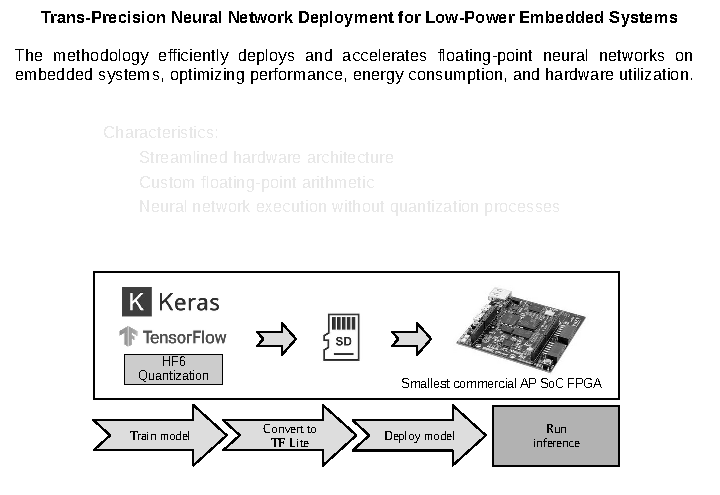
\includegraphics[width=\textwidth]{slides/Methodlogy/1.pdf}}
	\only<2>{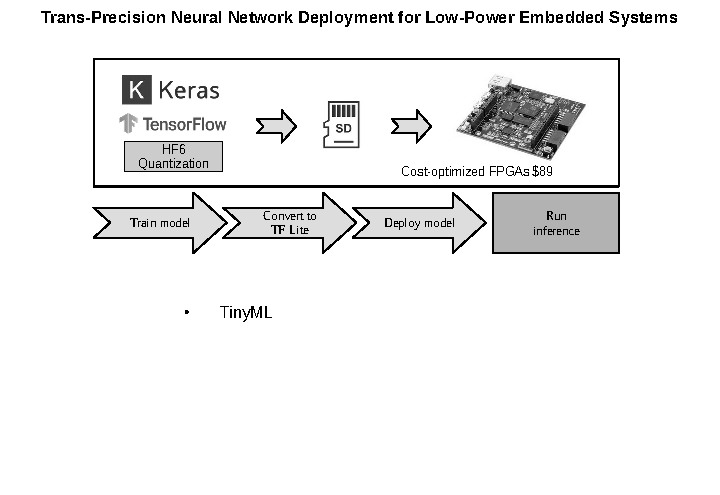
\includegraphics[width=\textwidth]{slides/Methodlogy/2.pdf}}
	\only<3>{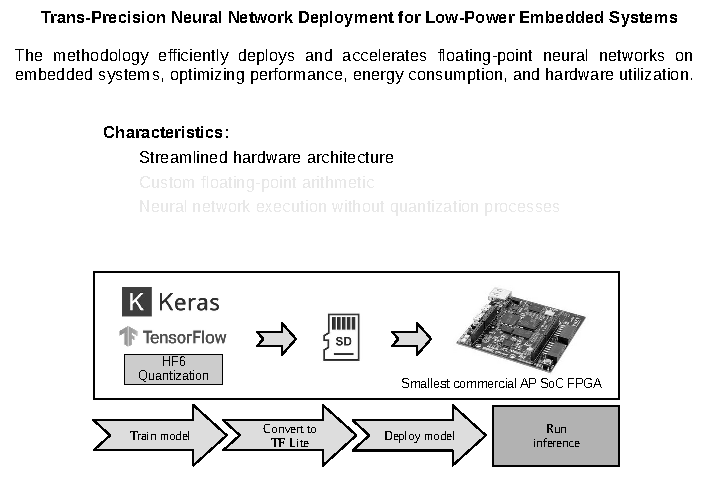
\includegraphics[width=\textwidth]{slides/Methodlogy/3.pdf}}
	\only<4>{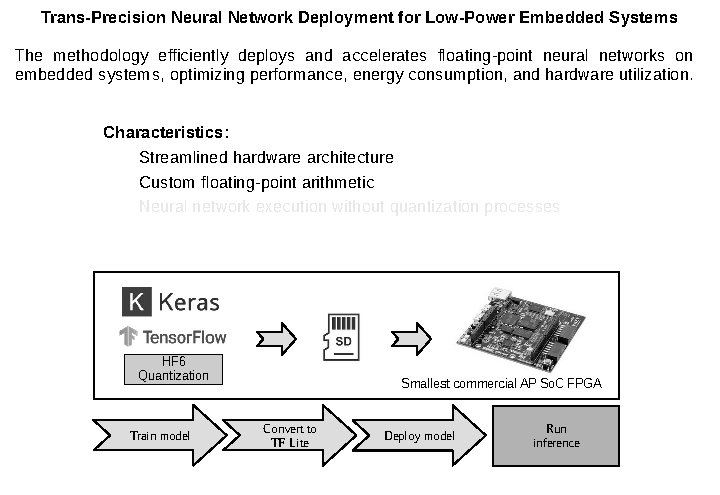
\includegraphics[width=\textwidth]{slides/Methodlogy/4.pdf}}
	\only<5>{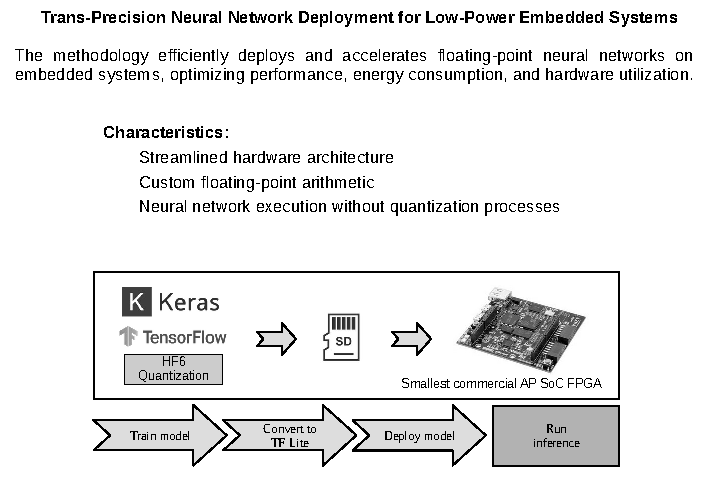
\includegraphics[width=\textwidth]{slides/Methodlogy/5.pdf}}
	\only<6>{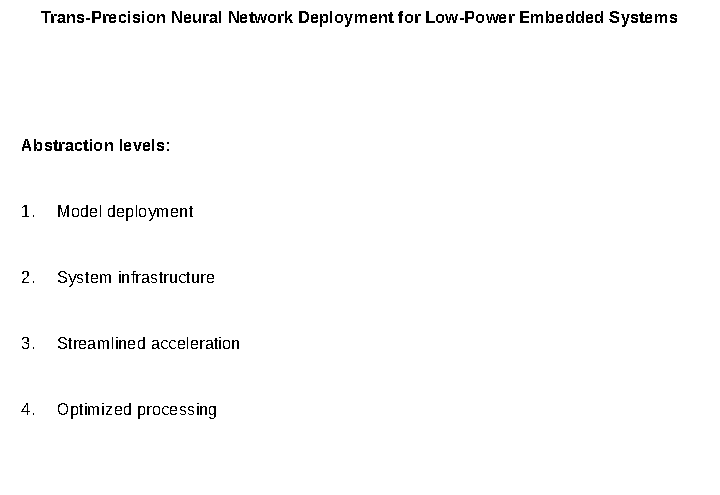
\includegraphics[width=\textwidth]{slides/Methodlogy/6.pdf}}
	\only<7>{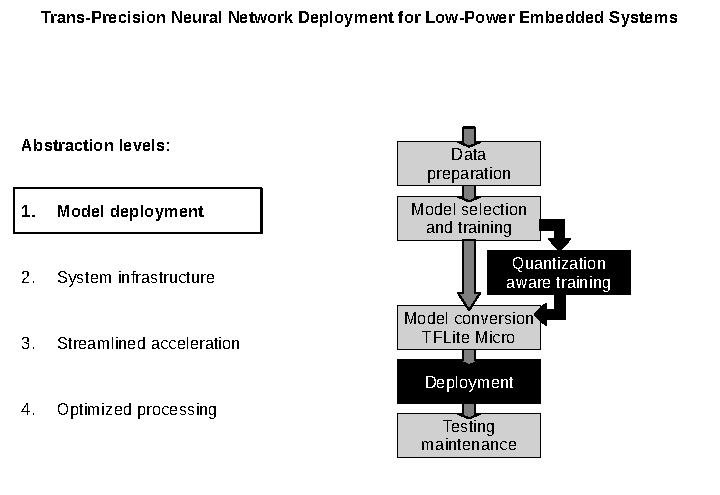
\includegraphics[width=\textwidth]{slides/Methodlogy/7.pdf}}
	\only<8>{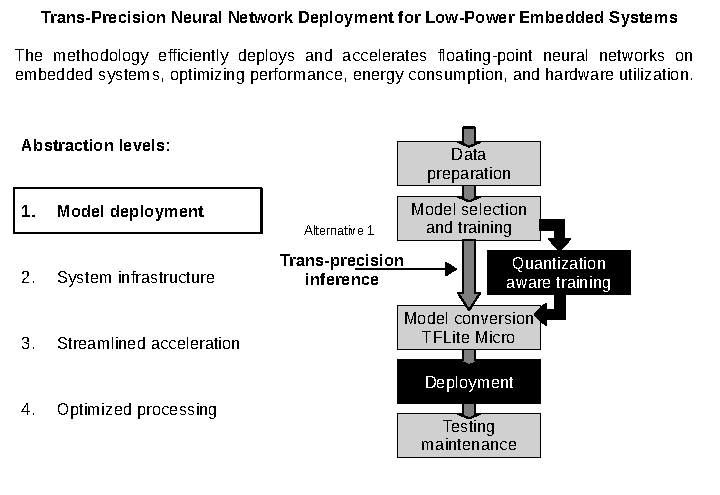
\includegraphics[width=\textwidth]{slides/Methodlogy/8.pdf}}
	\only<9>{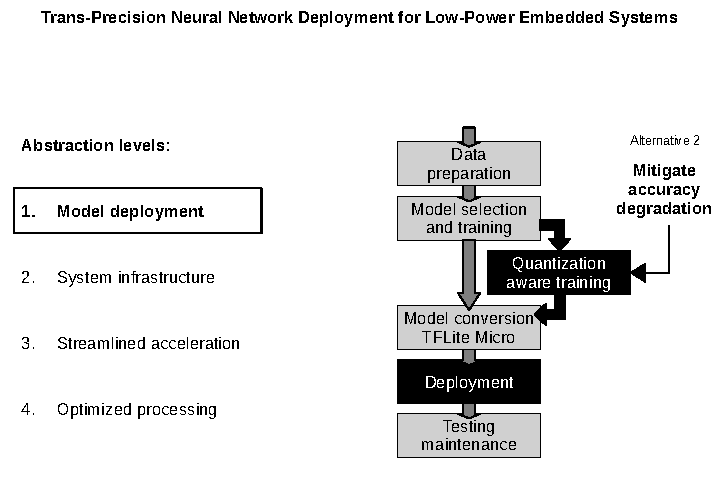
\includegraphics[width=\textwidth]{slides/Methodlogy/9.pdf}}
	\only<10>{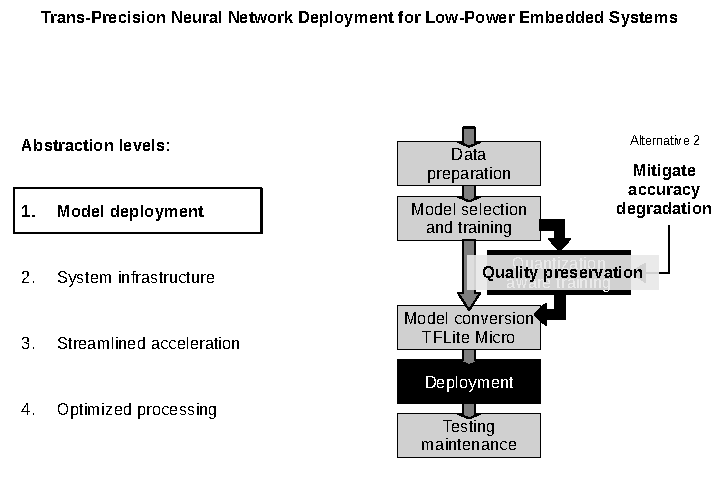
\includegraphics[width=\textwidth]{slides/Methodlogy/10.pdf}}
	\only<11>{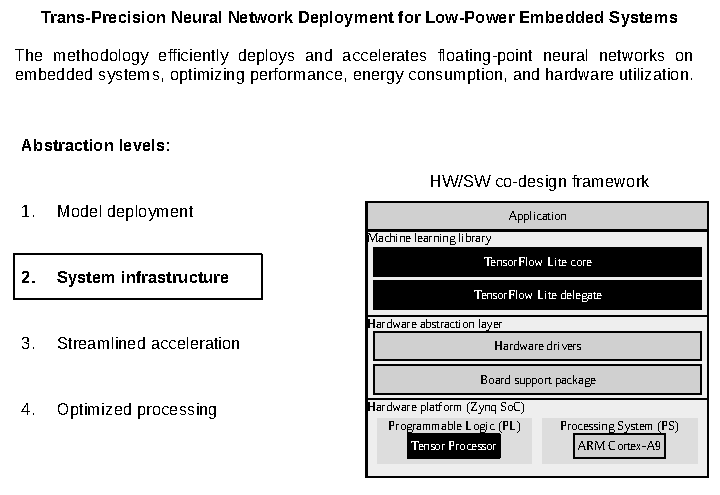
\includegraphics[width=\textwidth]{slides/Methodlogy/11.pdf}}
	\only<12>{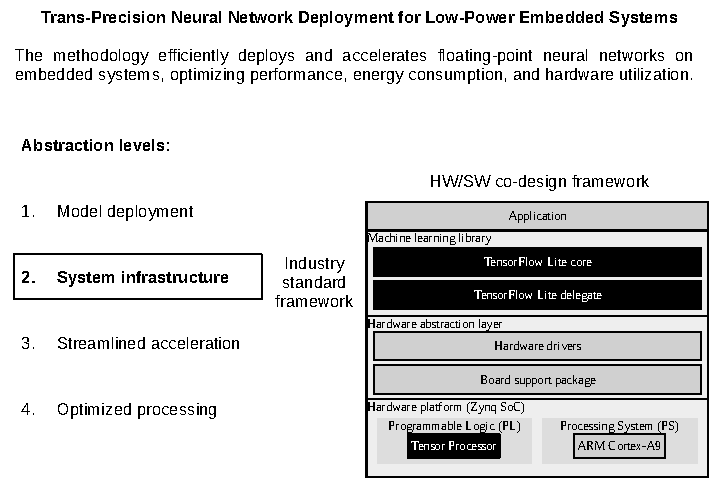
\includegraphics[width=\textwidth]{slides/Methodlogy/12.pdf}}
	\only<13>{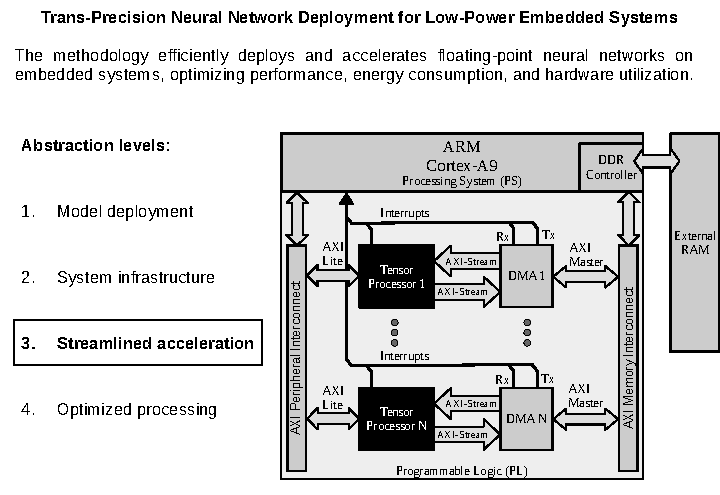
\includegraphics[width=\textwidth]{slides/Methodlogy/13.pdf}}
	\only<14>{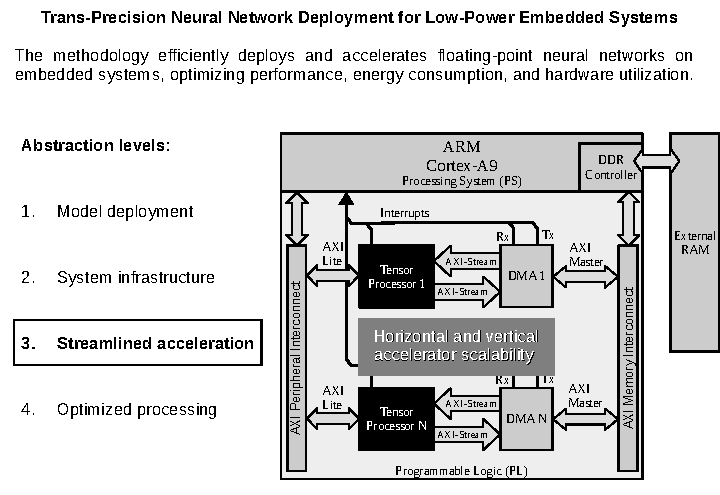
\includegraphics[width=\textwidth]{slides/Methodlogy/14.pdf}}
	\only<15>{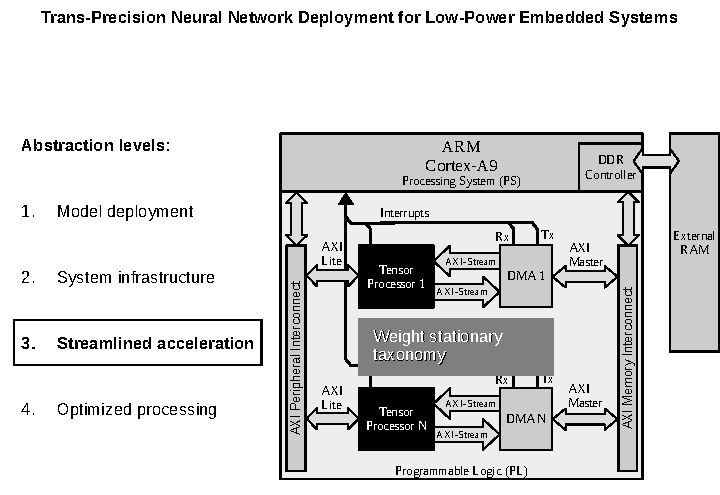
\includegraphics[width=\textwidth]{slides/Methodlogy/15.pdf}}
	\only<16>{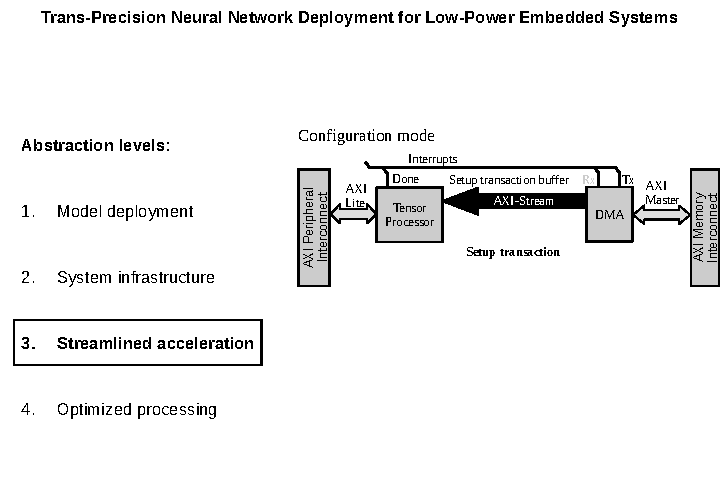
\includegraphics[width=\textwidth]{slides/Methodlogy/16.pdf}}
	\only<17>{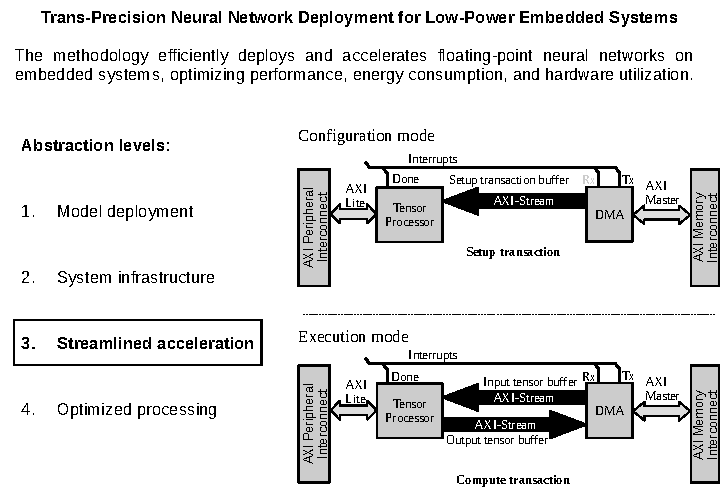
\includegraphics[width=\textwidth]{slides/Methodlogy/17.pdf}}
	\only<18>{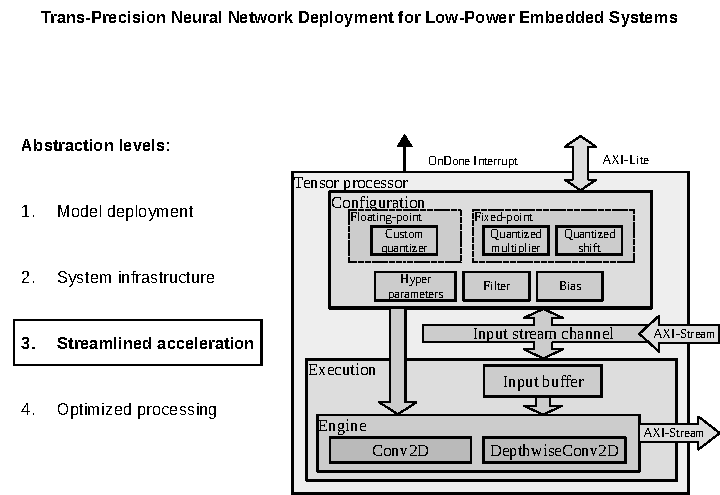
\includegraphics[width=\textwidth]{slides/Methodlogy/18.pdf}}
	\only<19>{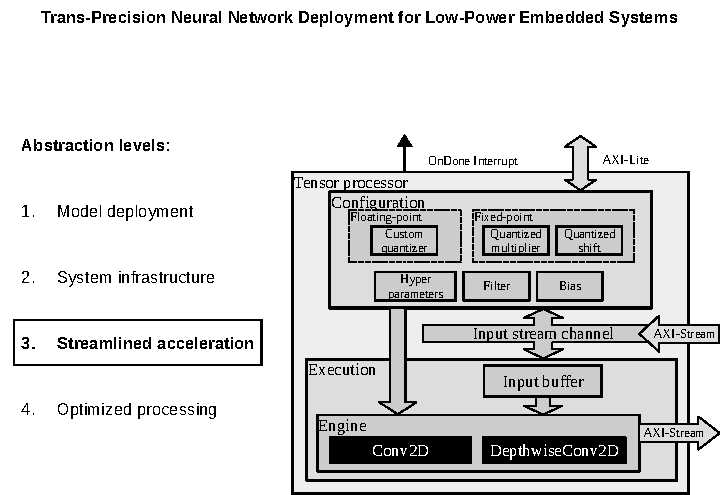
\includegraphics[width=\textwidth]{slides/Methodlogy/19.pdf}}
	\only<20>{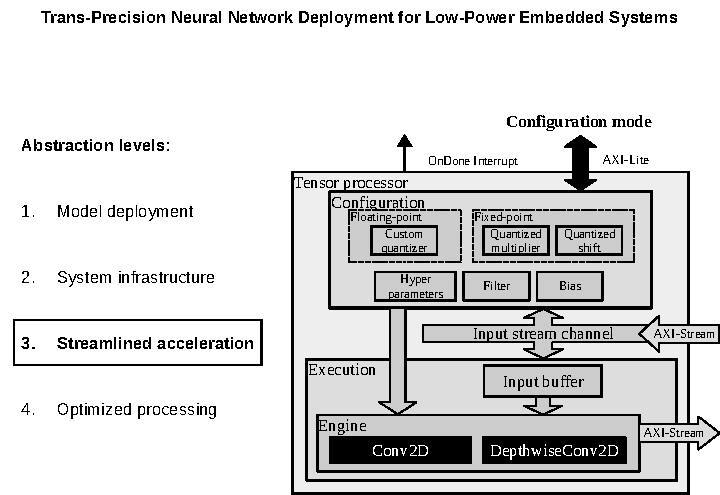
\includegraphics[width=\textwidth]{slides/Methodlogy/20.pdf}}
	\only<21>{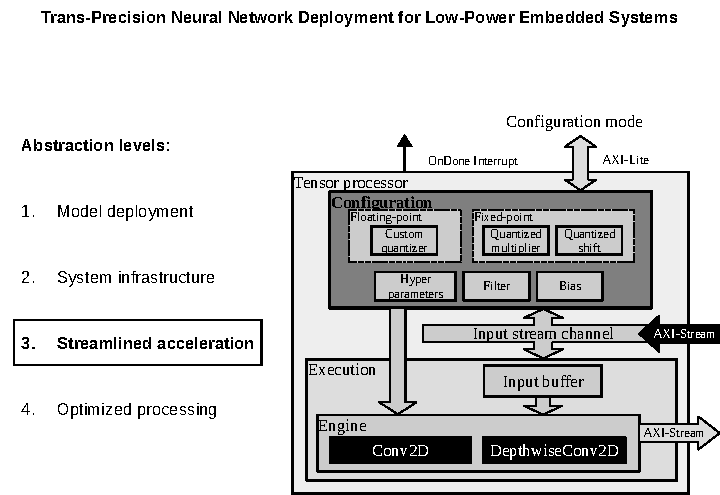
\includegraphics[width=\textwidth]{slides/Methodlogy/21.pdf}}
	\only<22>{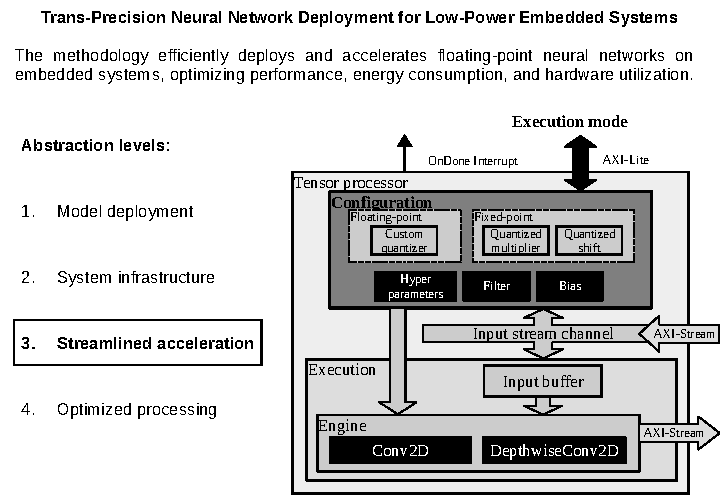
\includegraphics[width=\textwidth]{slides/Methodlogy/22.pdf}}
	\only<23>{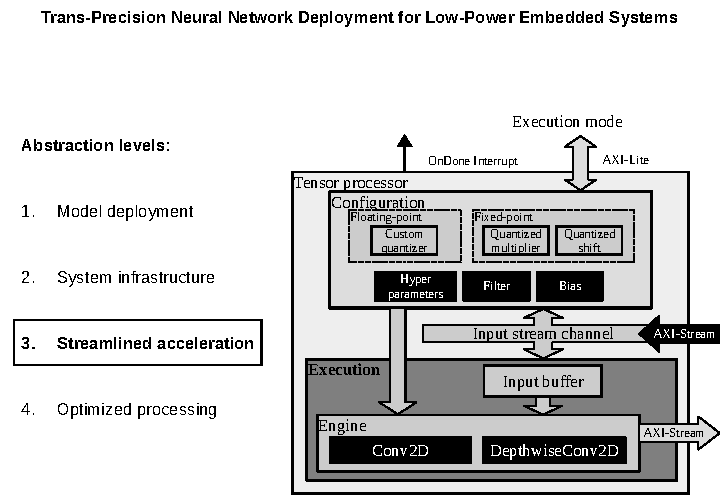
\includegraphics[width=\textwidth]{slides/Methodlogy/23.pdf}}
	\only<24>{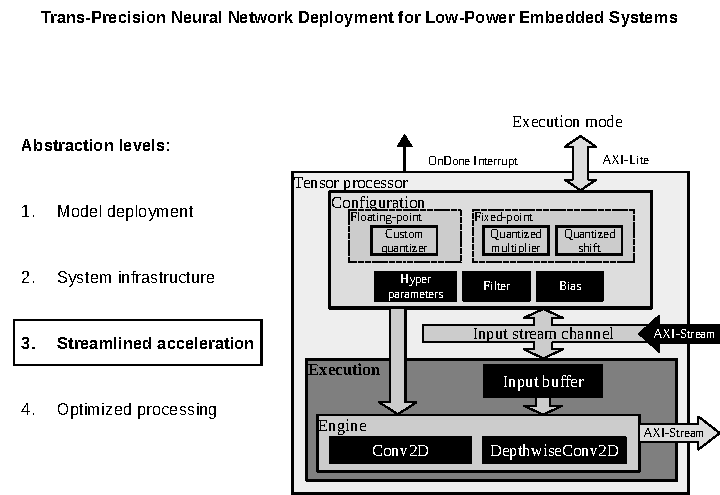
\includegraphics[width=\textwidth]{slides/Methodlogy/24.pdf}}
	\only<25>{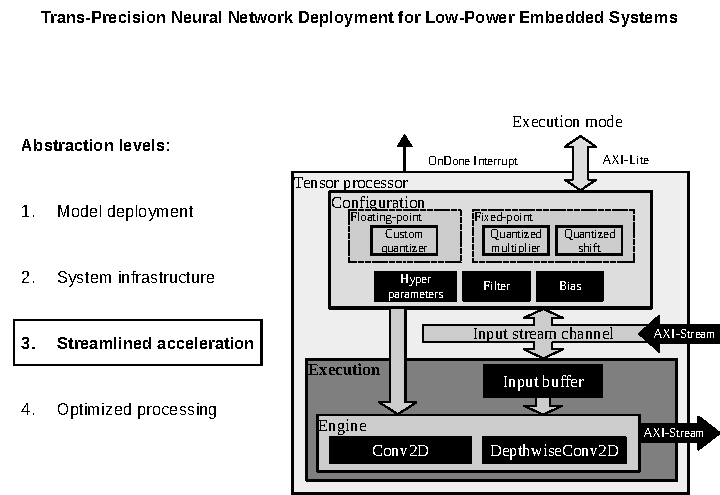
\includegraphics[width=\textwidth]{slides/Methodlogy/25.pdf}}
	\only<26>{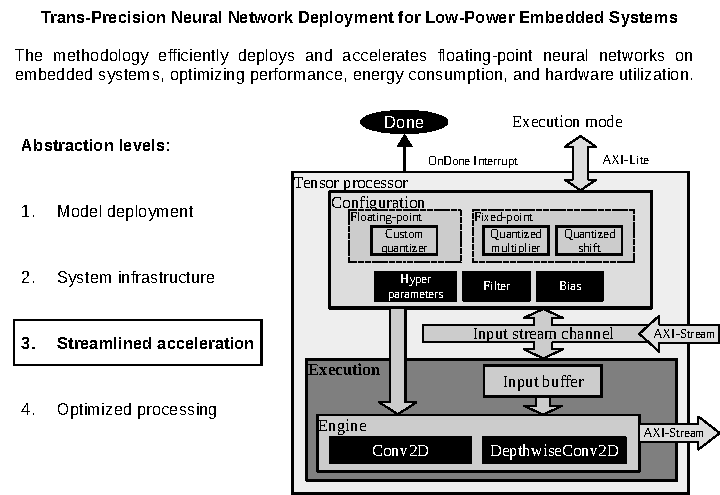
\includegraphics[width=\textwidth]{slides/Methodlogy/26.pdf}}
	
	%\only<27>{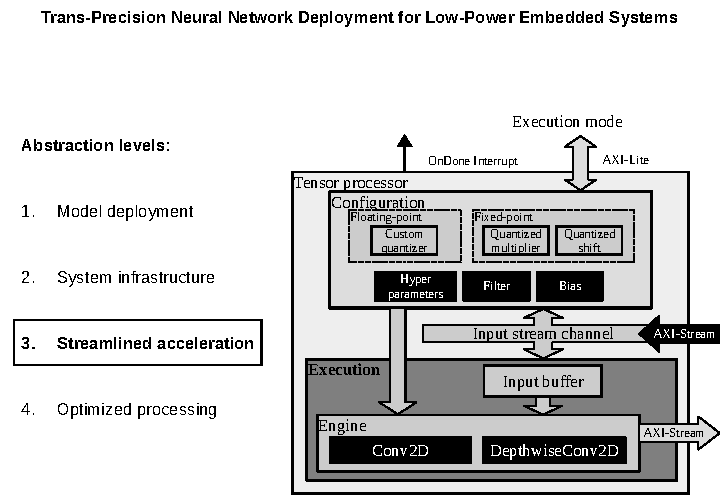
\includegraphics[width=\textwidth]{slides/Methodlogy/23.pdf}}
	%\only<28>{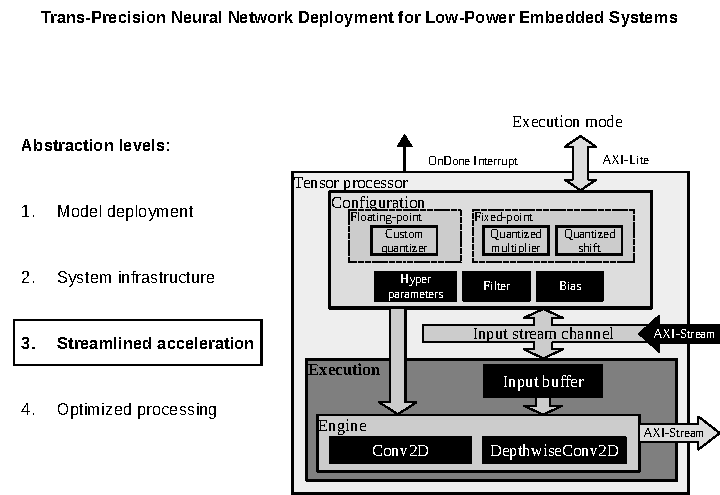
\includegraphics[width=\textwidth]{slides/Methodlogy/24.pdf}}
	%\only<29>{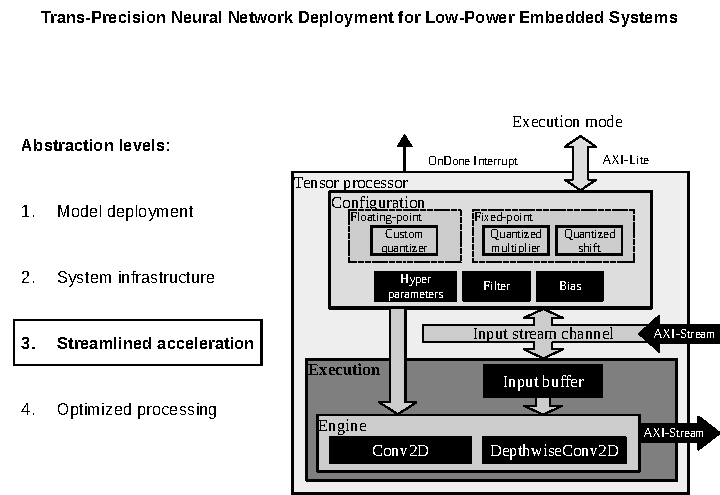
\includegraphics[width=\textwidth]{slides/Methodlogy/25.pdf}}
	%\only<30>{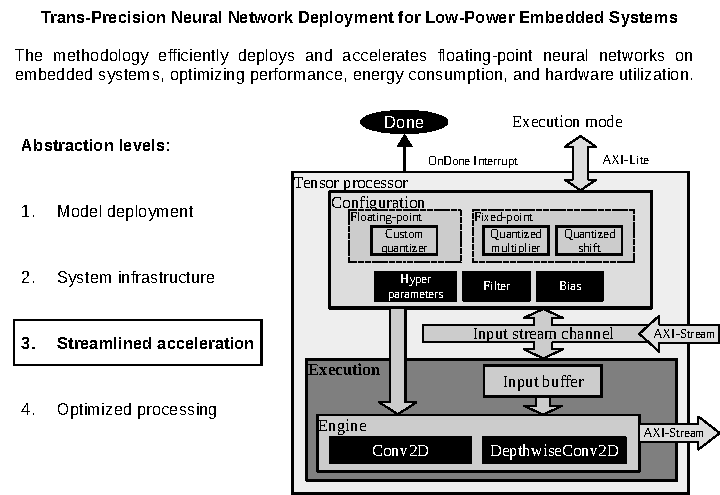
\includegraphics[width=\textwidth]{slides/Methodlogy/26.pdf}}
	
	\only<27>{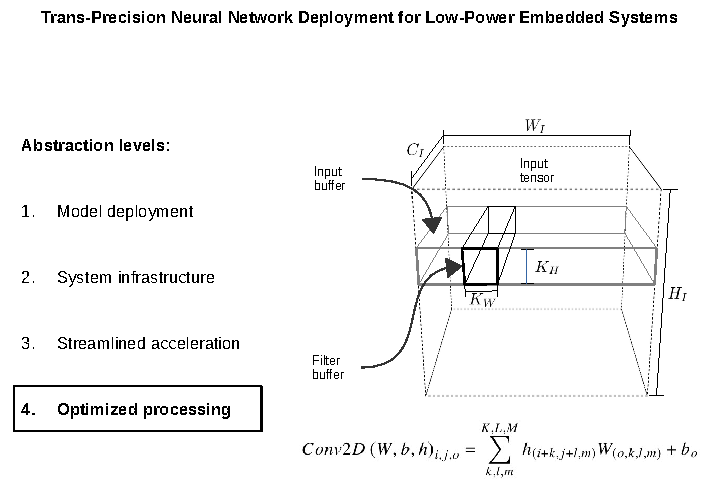
\includegraphics[width=\textwidth]{slides/Methodlogy/31.pdf}}
	\only<28>{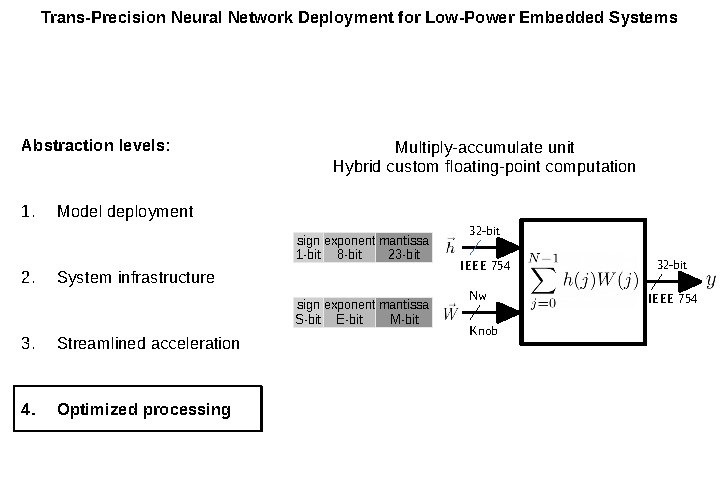
\includegraphics[width=\textwidth]{slides/Methodlogy/32.pdf}}
	\only<29>{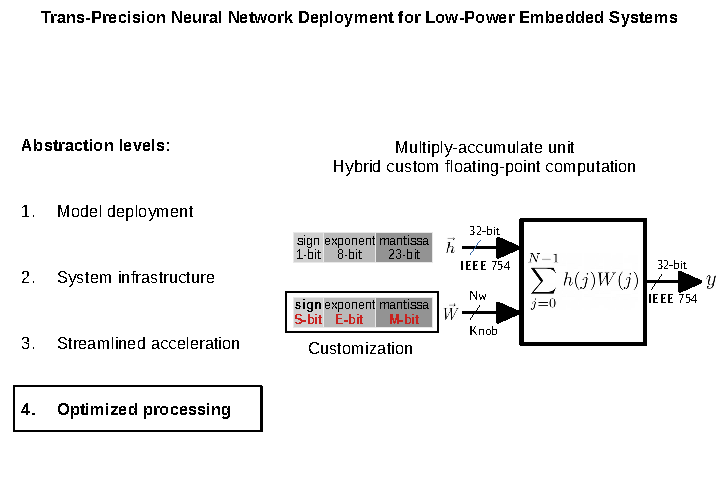
\includegraphics[width=\textwidth]{slides/Methodlogy/33.pdf}}
	\only<30>{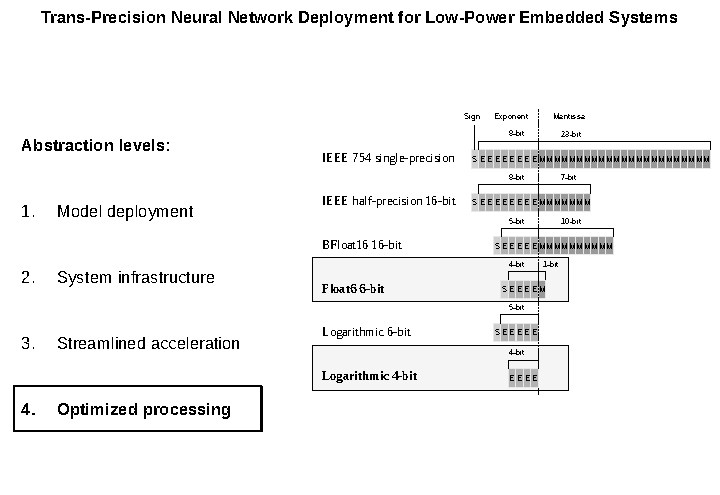
\includegraphics[width=\textwidth]{slides/Methodlogy/34.pdf}}
	%\only<31>{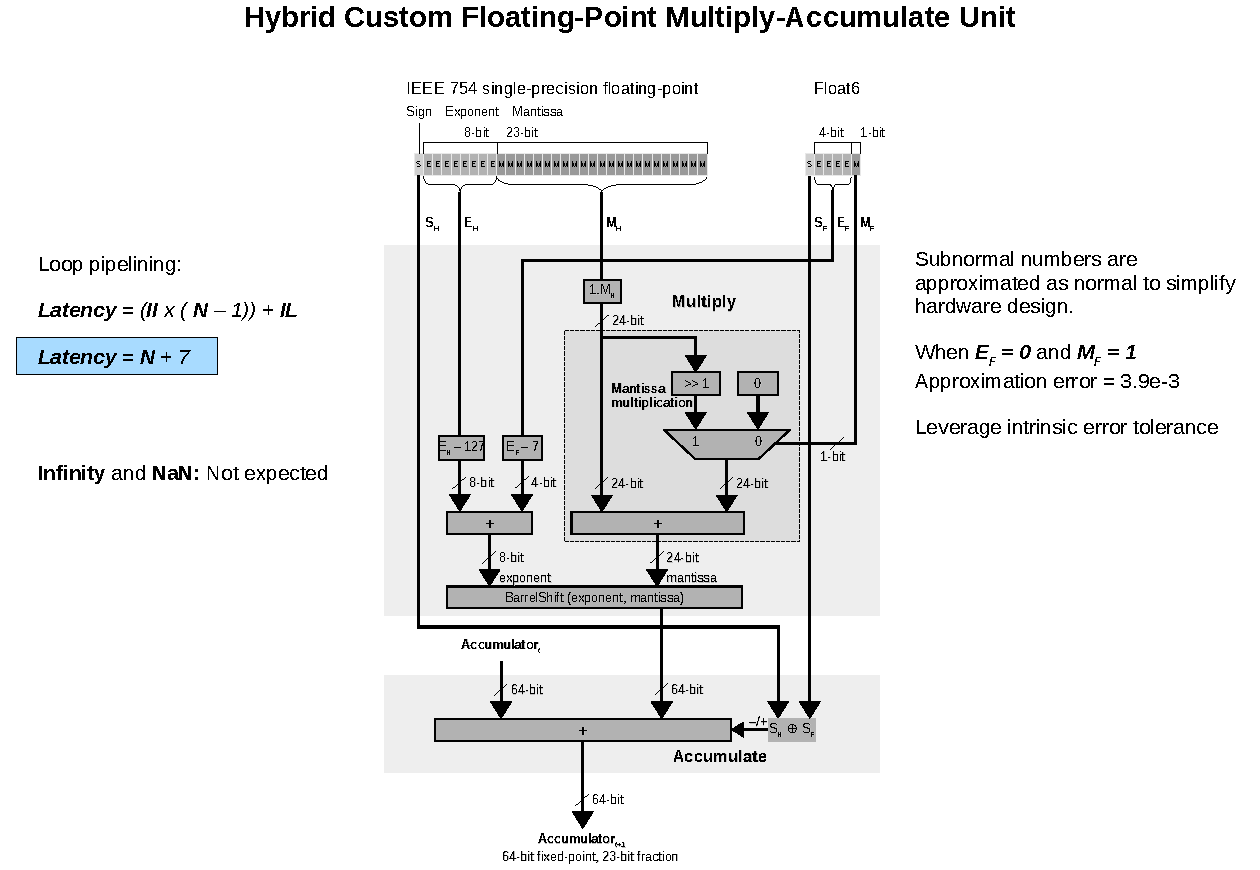
\includegraphics[width=\textwidth]{slides/Methodlogy/mac.pdf}}
	%\only<32>{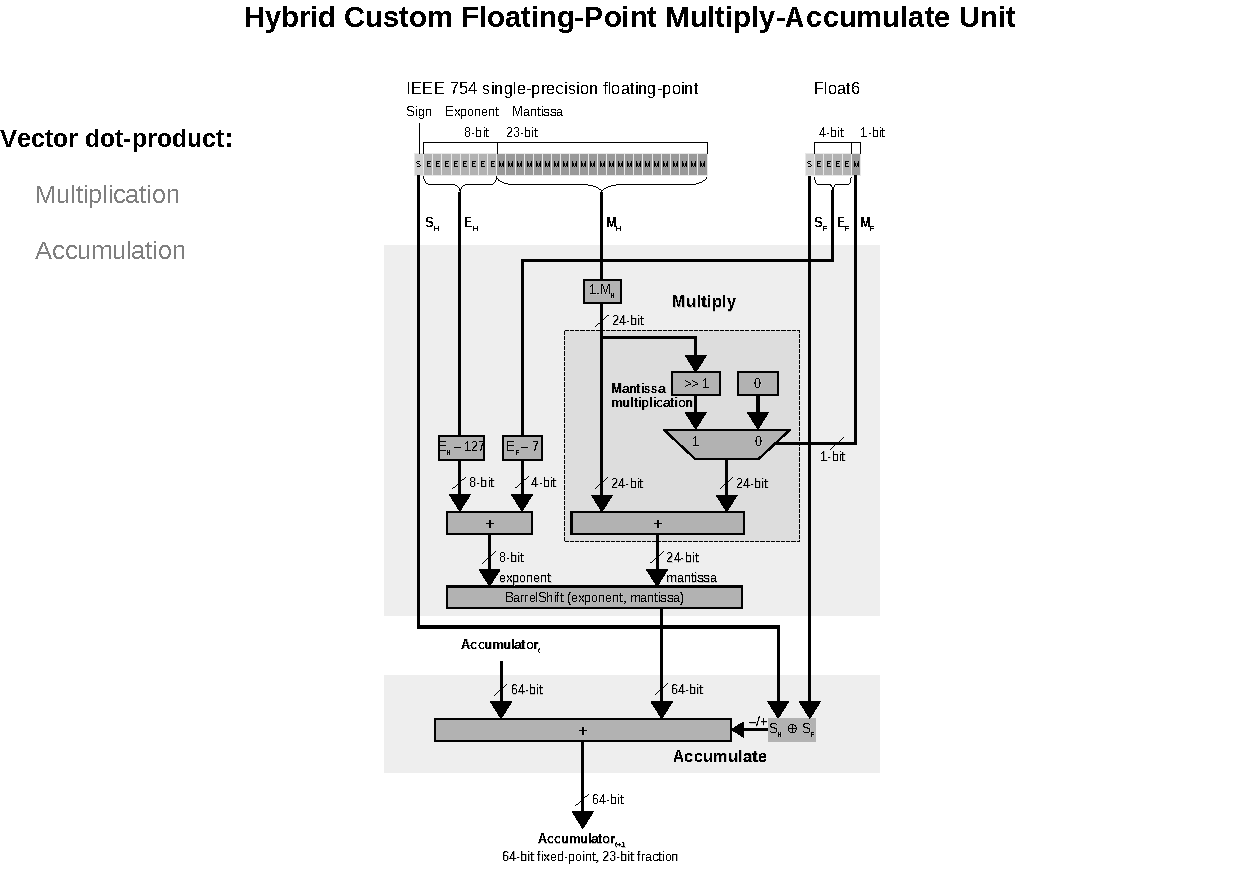
\includegraphics[width=\textwidth]{slides/Methodlogy/mac-2.pdf}}
	%\only<33>{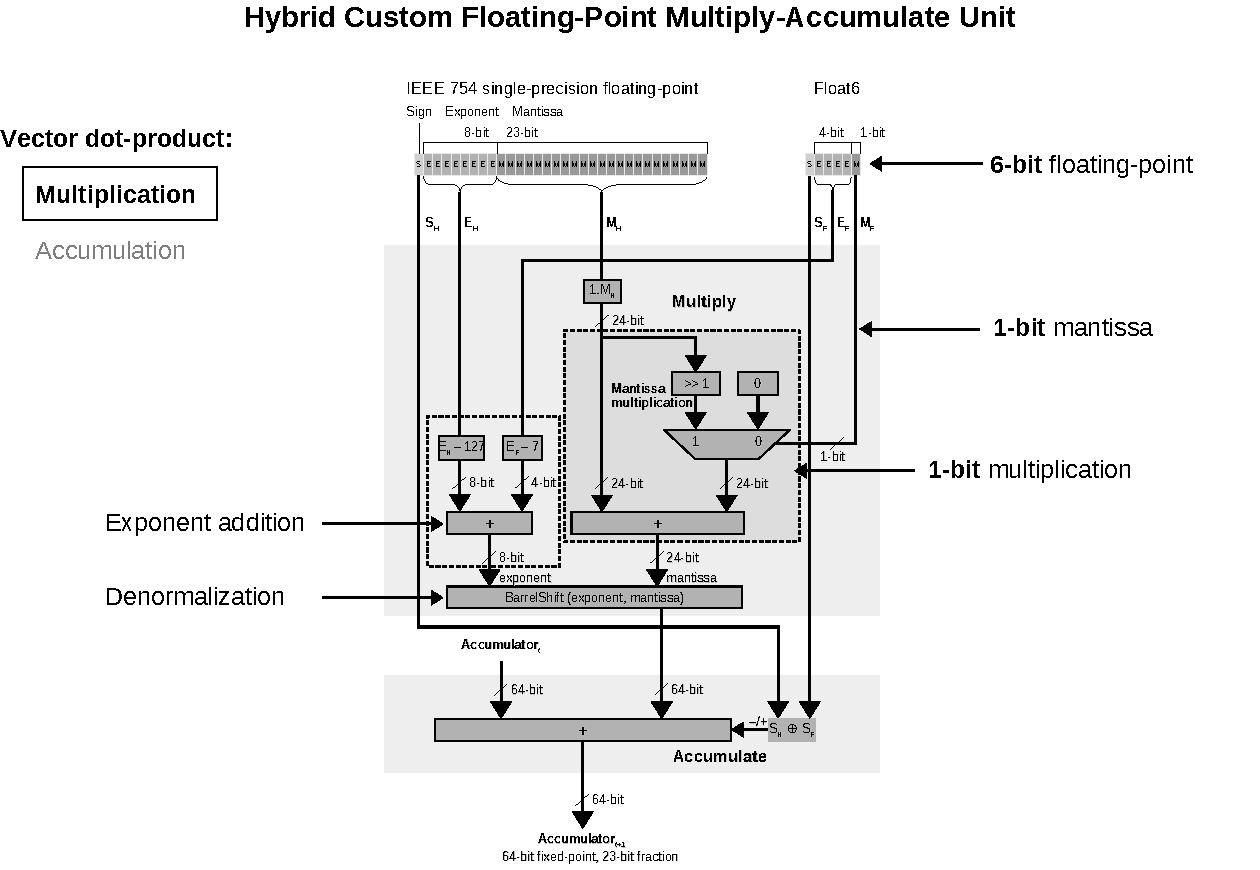
\includegraphics[width=\textwidth]{slides/Methodlogy/mac-3.pdf}}
	%\only<34>{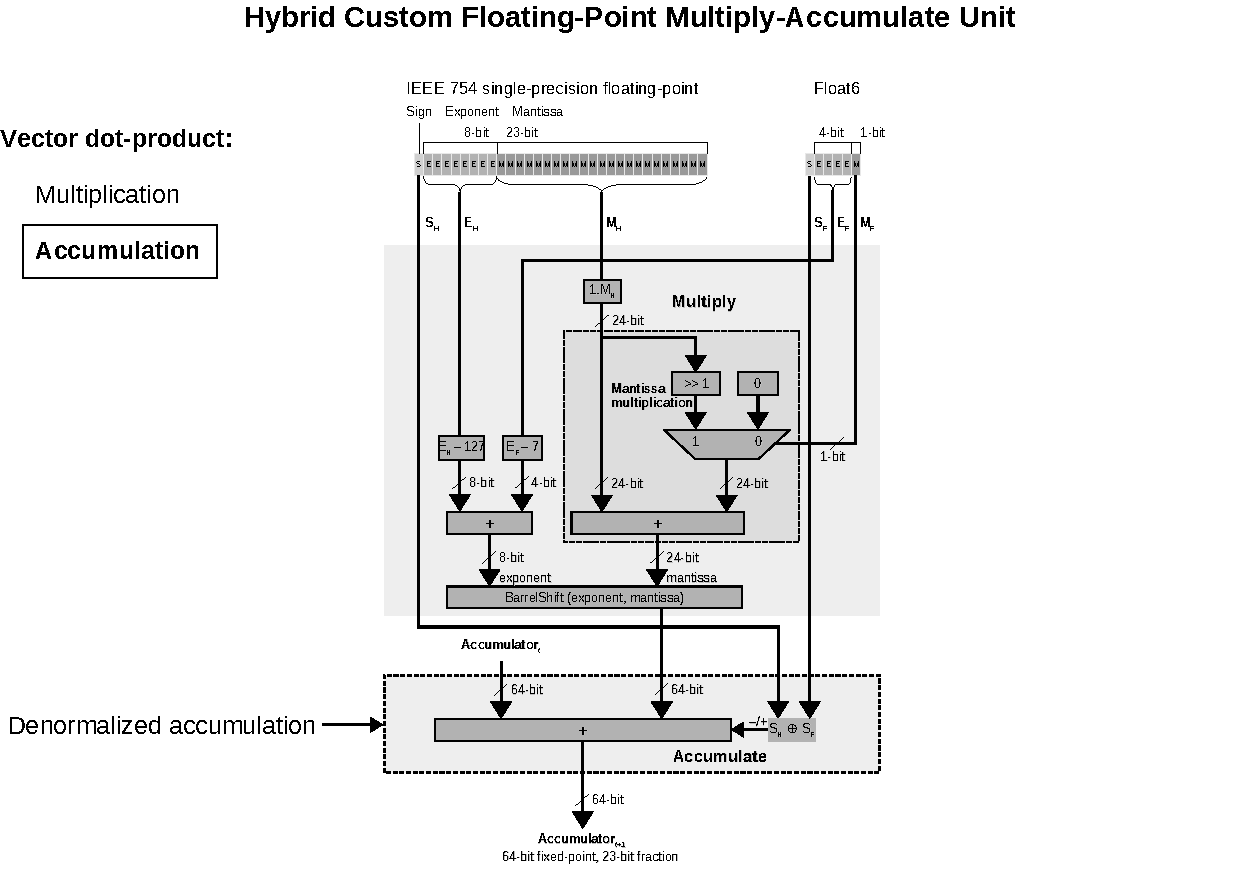
\includegraphics[width=\textwidth]{slides/Methodlogy/mac-4.pdf}}
	%\only<35>{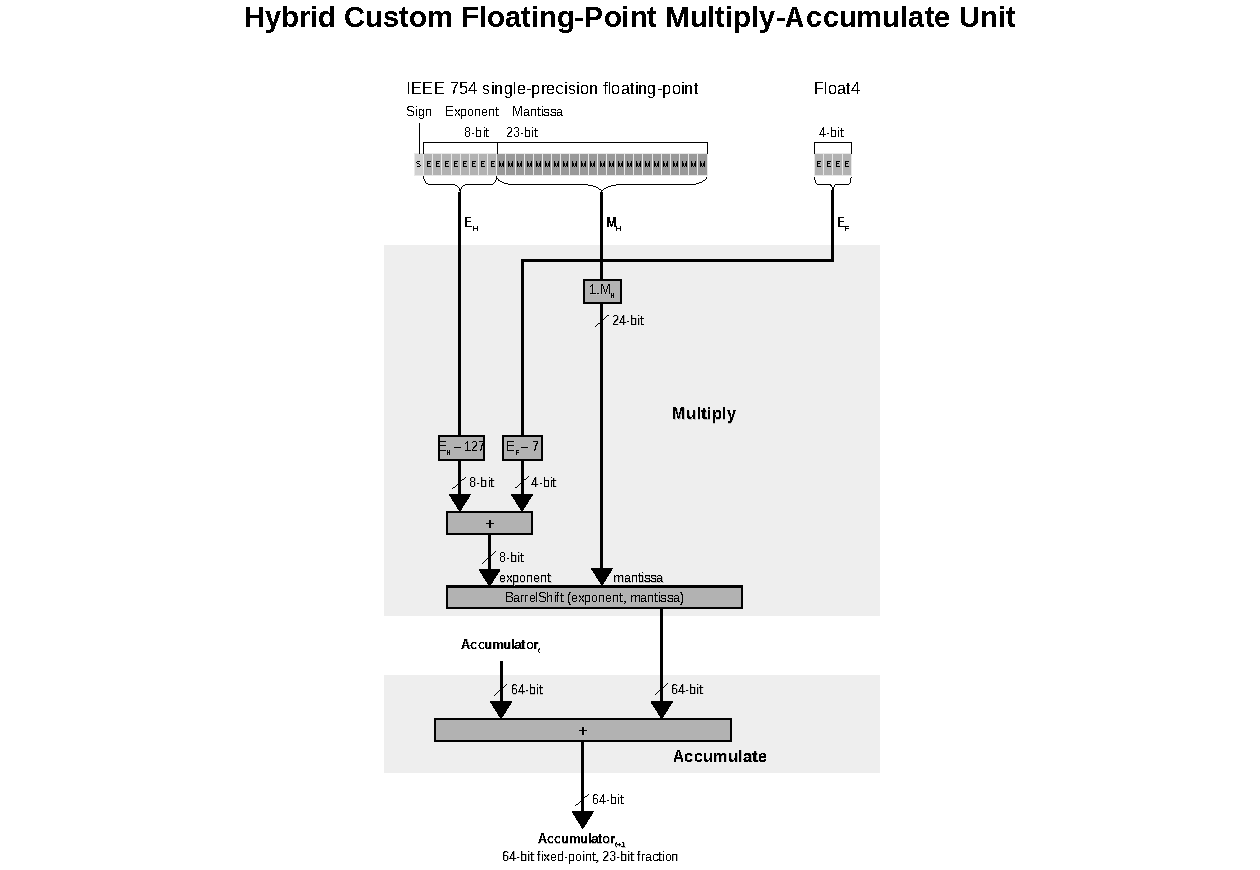
\includegraphics[width=\textwidth]{slides/Methodlogy/mac-5.pdf}}
	%\only<36>{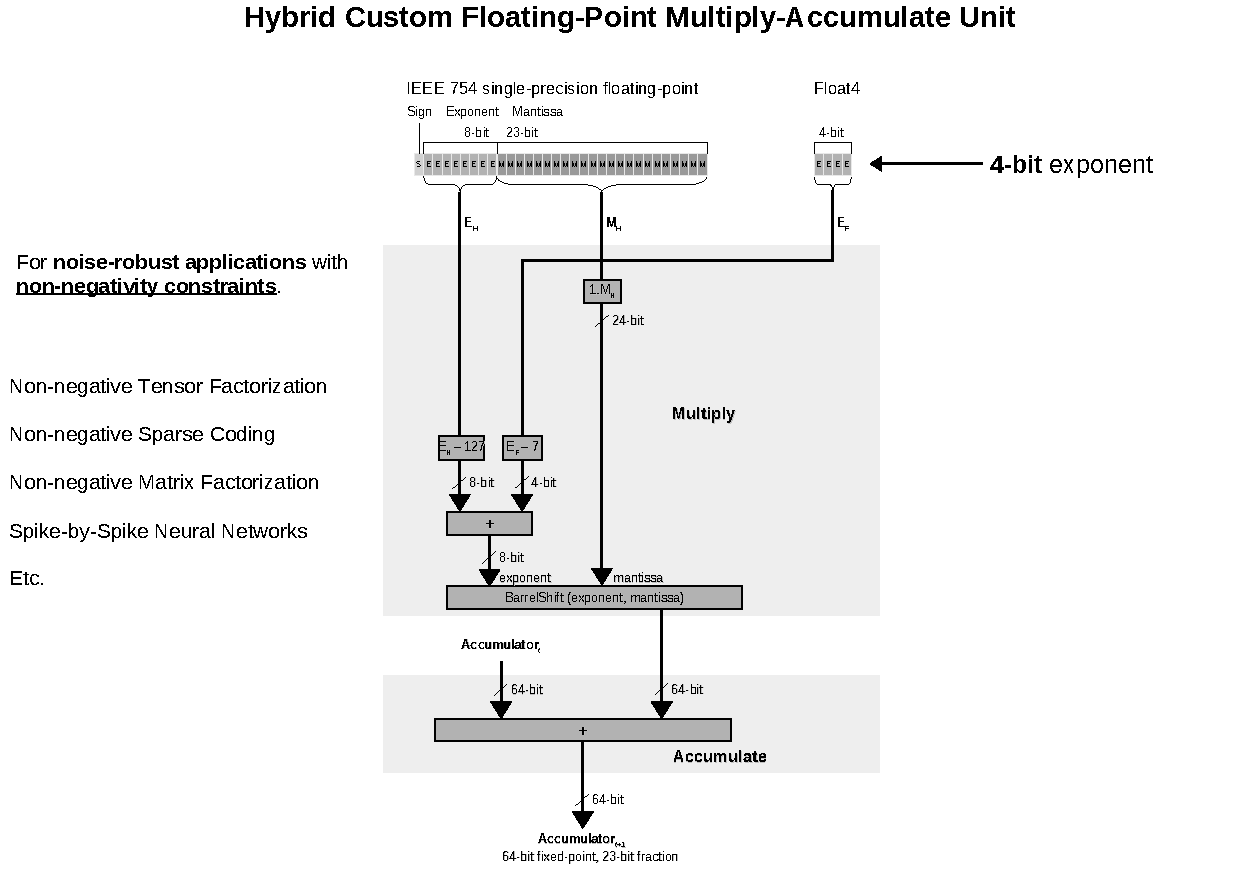
\includegraphics[width=\textwidth]{slides/Methodlogy/mac-6.pdf}}
	%\only<37>{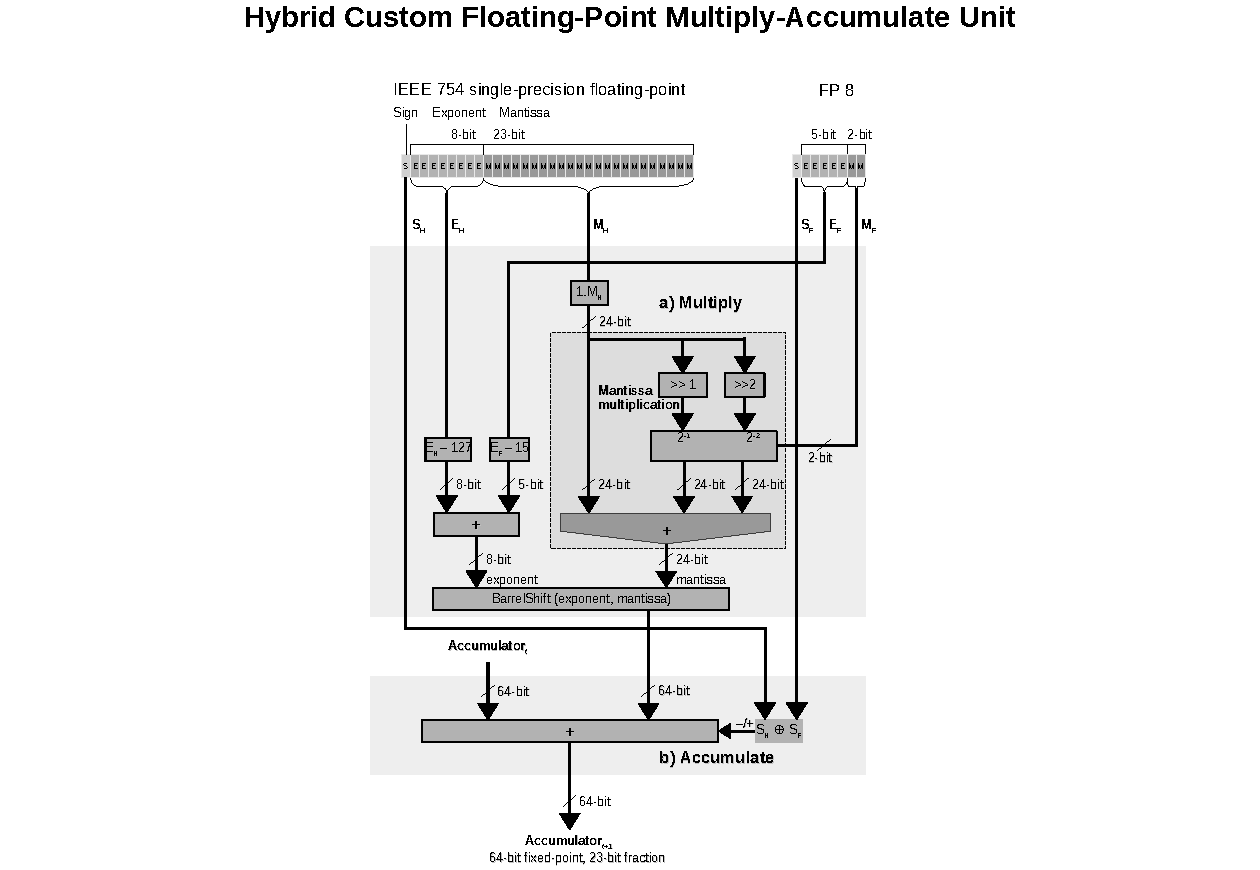
\includegraphics[width=\textwidth]{slides/Methodlogy/mac-7.pdf}}
	%\only<37>{\centering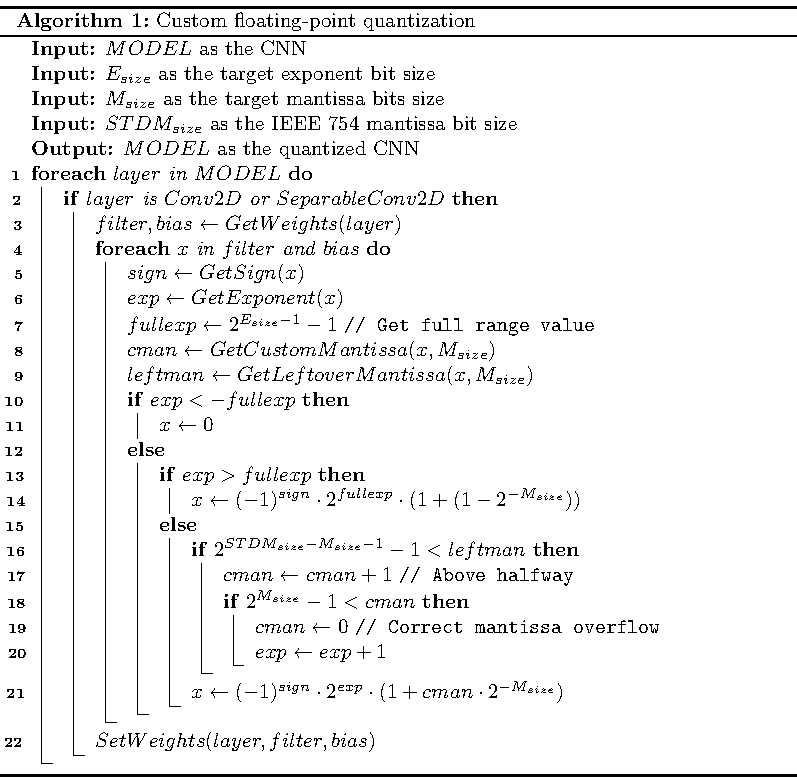
\includegraphics[width=0.7\textwidth]{slides/Methodlogy/qat.pdf}}
\end{frame}
	
	\section{Hybrid 8-bit Floating-Point and 4-bit Logarithmic Computation}
\tableofcontents[currentsection]
\begin{frame}{Spike-by-Spike Neural Network}
	\begin{columns}[c] % The [T] option aligns the tops of the columns
		
		% Left column for the first image
		\begin{column}<1->{0.5\textwidth}
			\begin{figure}
				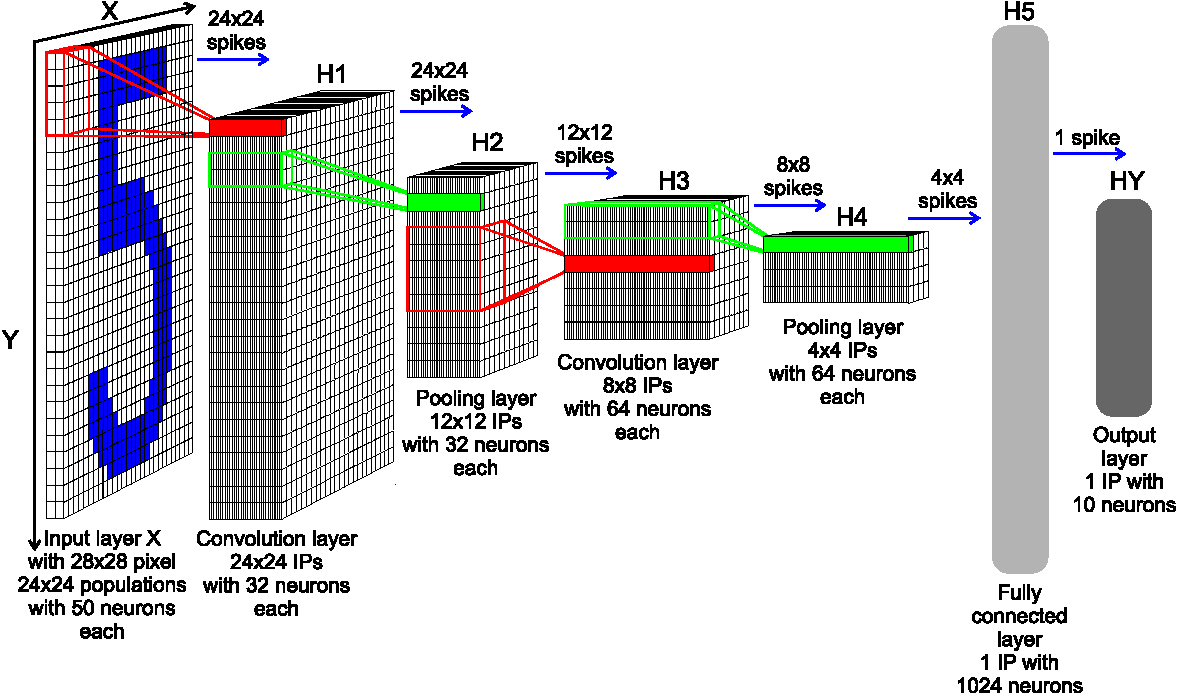
\includegraphics[width=\textwidth]{../chapters/sbs_accelerator/figures/sbs_network.pdf} % Adjust the filename
				\caption{\scriptsize Spike-by-Spike (SbS) neural network architecture for handwritten digit classification task.}
			\end{figure}
		\end{column}
		
		% Right column for the second image
		\begin{column}<2->{0.5\textwidth}
			\begin{figure}
				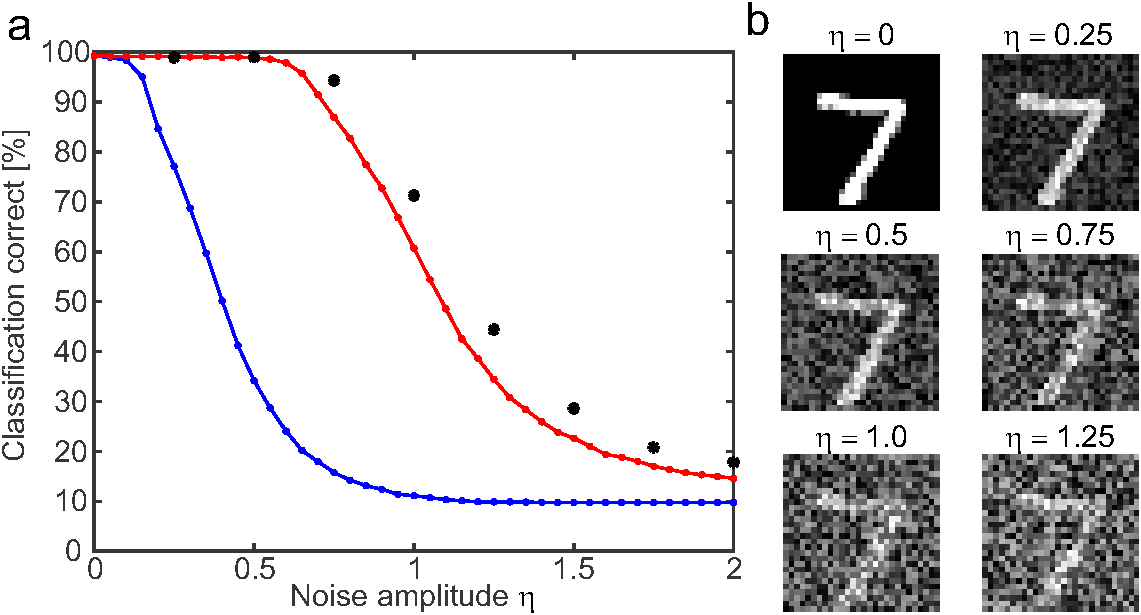
\includegraphics[width=\textwidth]{../chapters/sbs_accelerator/figures/sbs_robustnes.pdf} % Adjust the filename
				\caption{\scriptsize Performance classification of SbS NN versus equivalent CNN.}
			\end{figure}
		\end{column}
		
	\end{columns}
\end{frame}

\begin{frame}{Spike-by-Spike Layer Update}
	\begin{figure}
		\centering
		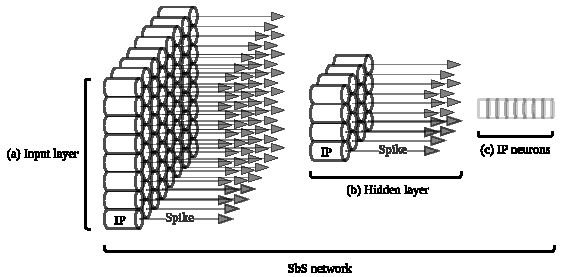
\includegraphics[width=0.5\textwidth]{../chapters/sbs_accelerator/figures/SbS_layer.pdf}
		\caption{\scriptsize SbS inference population (IP) as independent computational entities.}
	\end{figure}
	
	%\pause % Pause for the equation to appear after the image
	
	% Equation at the bottom
	{\scriptsize
		\[
		h_\mu^{new}(i) = \frac{1}{1+\epsilon} \left(h_\mu(i) + \epsilon \frac{h_\mu(i) W(s_t|i) }{\sum_j h_\mu(j) W(s_t|j)} \right) 
		\]
	}
\end{frame}

\begin{frame}{HW/SW Co-Design Framework}
	\begin{columns}[t] % The [T] option aligns the tops of the columns
		
		% Left column for the first image
		\begin{column}{0.5\textwidth}
			\begin{figure}
				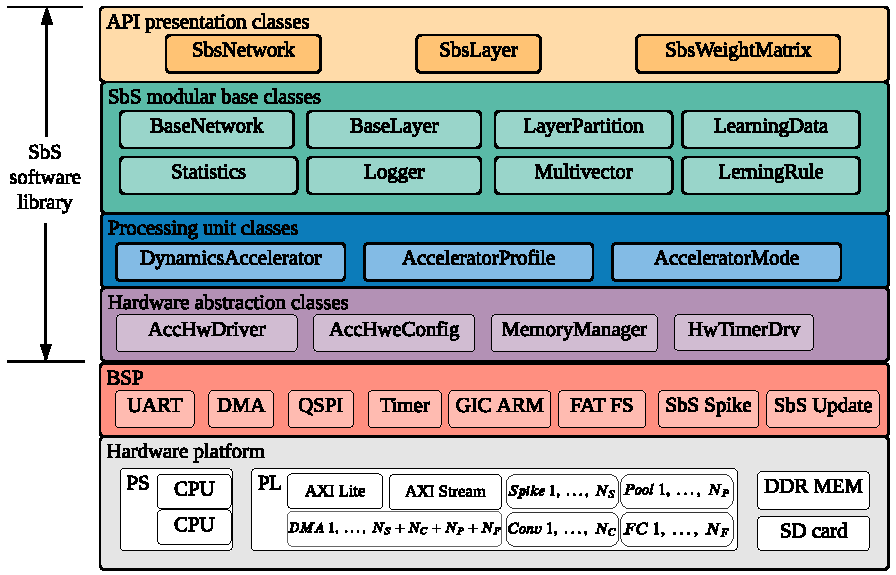
\includegraphics[width=0.8\textwidth]{../chapters/sbs_accelerator/figures/sbs_software_component.pdf}
				\caption{\scriptsize System-level overview of the embedded software architecture.}
			\end{figure}
		\end{column}
		
		% Right column for the second image
		\begin{column}{0.5\textwidth}
			\begin{figure}
				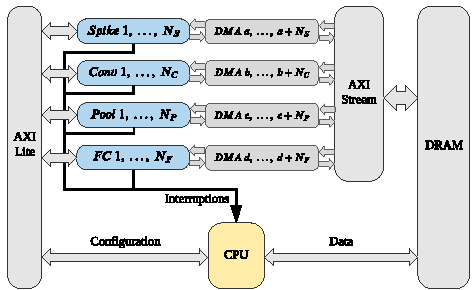
\includegraphics[width=0.8\textwidth]{../chapters/sbs_accelerator/figures/sbs_hw.pdf} % Adjust the filename
				\caption{\scriptsize System-level hardware architecture with scalable number of heterogeneous processing units (PU).}
			\end{figure}
		\end{column}
		
	\end{columns}
\end{frame}

\begin{frame}{Processing Unit}
	\begin{columns}[c] % The [T] option aligns the tops of the columns
		
		% Left column for the first image
		\begin{column}<1->{0.5\textwidth}
			\begin{figure}
				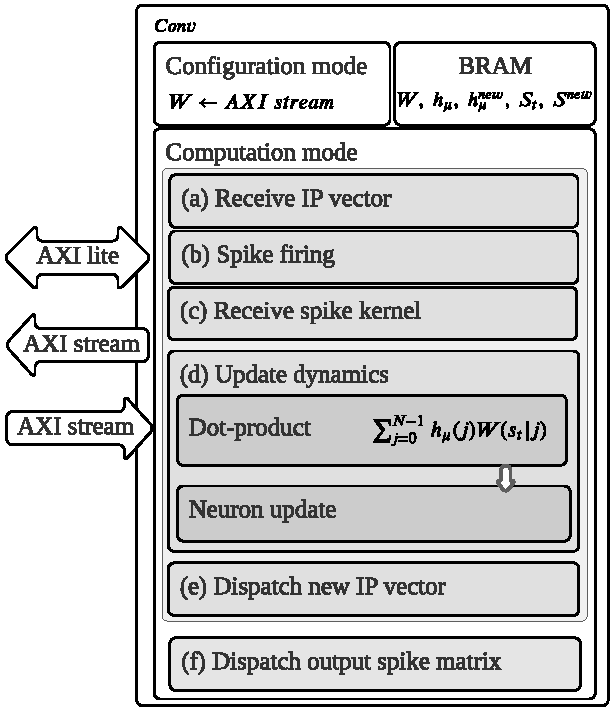
\includegraphics[width=0.7\textwidth]{../chapters/sbs_accelerator/figures/sbs_conv.pdf} % Adjust the filename
				\caption{\scriptsize Conv processing unit.}
			\end{figure}
		\end{column}
		
		% Right column for the second image
		\begin{column}<2->{0.5\textwidth}
			\begin{figure}
				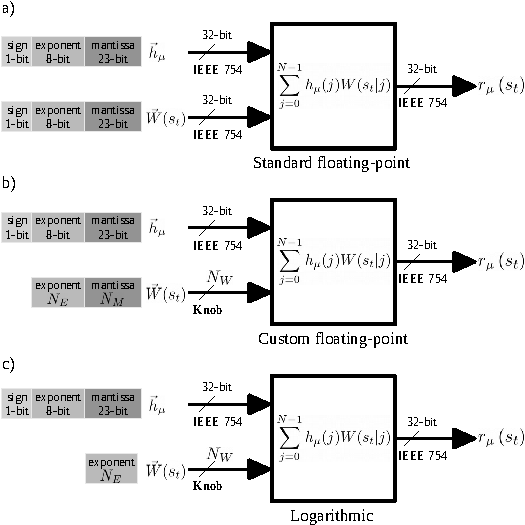
\includegraphics[width=0.9\textwidth]{../chapters/sbs_accelerator/figures/dot-product_unit.pdf} % Adjust the filename
				\caption{\scriptsize Dot-product hardware module.}
			\end{figure}
		\end{column}
		
	\end{columns}
\end{frame}

\begin{frame}{Hybrid Dot-Product Approximation}
	\begin{columns}[c] % The [T] option aligns the tops of the columns
		% Left column for equations
		\begin{column}{0.5\textwidth}
			\scriptsize
			\vspace{5mm}
			\begin{equation}
			r_{\mu}\left(s_t\right)=\sum_{j=0}^{N-1}h_{\mu}(j)W(s_t|j)
			\end{equation}
			\vspace{5mm} 
			\begin{equation}
			E_{\min}=\log _2(\min_{\forall i}(W(i)))
			\end{equation}
			\vspace{5mm} 
			\begin{equation}
			N_E=\lceil\log_2(|E_{\min}|)\rceil
			\end{equation}
			\vspace{5mm} 
			\begin{equation}
			N_W=N_E + N_M
			\end{equation}
		\end{column}
		
		% Right column for the image
		\begin{column}{0.5\textwidth}
			\begin{figure}
				\centering
				\includegraphics[width=0.9\textwidth]{../chapters/sbs_accelerator/figures/dot-product_unit.pdf} % Adjust the filename
				\caption{\scriptsize Dot-product hardware module.}
			\end{figure}
		\end{column}
	\end{columns}
\end{frame}

\begin{frame}{Dot-Product with Standard Floating-Point (IEEE 754)}
	\begin{figure}
		\centering
		\includegraphics[width=0.4\columnwidth]{../chapters/sbs_accelerator/figures/dot_product_float.pdf}
		\caption{\scriptsize Dot-product hardware module with standard floating-point computation.}
	\end{figure}
\scriptsize
	
	\vfill % Add vertical space to push the equation to the bottom
	
	% Equation at the bottom
	\[
	 L_{f32}=10N+9
	\]
\end{frame}

\begin{frame}{Dot-Product with Hybrid Custom Floating-Point Approximation}
	\begin{figure}
		\centering
		\includegraphics[width=0.4\columnwidth]{../chapters/sbs_accelerator/figures/dot_product.pdf}
		\caption{\scriptsize Dot-product hardware module with hybrid custom floating-point approximation.}
	\end{figure}
	\scriptsize
	
	\vfill % Add vertical space to push the equation to the bottom
	
	% Equation at the bottom
	\[
	L_{custom}=2N+11
	\]
\end{frame}

\begin{frame}{Dot-product with Hybrid Logarithmic Approximation}
	\begin{figure}
		\centering
		\includegraphics[width=0.4\columnwidth]{../chapters/sbs_accelerator/figures/dot_product_log.pdf}
		\caption{\scriptsize Dot-product hardware module with hybrid logarithmic approximation.}
	\end{figure}
	\scriptsize
	
	\vfill % Add vertical space to push the equation to the bottom
	
	% Equation at the bottom
	\[
	L_{custom}=2N+7
	\]
\end{frame}

\begin{frame}{Acceleration with Standard Floating-Point}
	\begin{columns}
		% Left Column
		\begin{column}{0.5\textwidth}
			% Top left image
			\begin{minipage}[c][.45\textheight][c]{\linewidth}
				\centering
				\begin{figure}
				\includegraphics[width=0.75\linewidth]{../chapters/sbs_accelerator/figures/sbs_hw_experimental.pdf} % Adjust path and size as needed
				\caption{\scriptsize System overview of the top-level architecture with 8 processing units.}
				\end{figure}
				\pause
			\end{minipage}
			
			% Bottom left image
			\begin{minipage}[c][.45\textheight][c]{\linewidth}
				\centering
				\begin{figure}
				\includegraphics[width=0.75\linewidth]{../chapters/sbs_accelerator/figures/latency_sw.pdf} % Adjust path and size as needed
				\caption{\scriptsize Computation on embedded CPU.}
				\end{figure}
				\pause
			\end{minipage}
		\end{column}
		
		% Right Column
		\begin{column}{0.5\textwidth}
			% Top right image
			\begin{minipage}[c][.45\textheight][c]{\linewidth}
				\centering
				\begin{figure}
				\includegraphics[width=0.75\linewidth]{../chapters/sbs_accelerator/figures/latency_pu_fp.pdf} % Adjust path and size as needed
				\caption{\scriptsize Performance of processing units with standard floating-point.}
				\end{figure}
				\pause
			\end{minipage}
			
			% Bottom right image
			\begin{minipage}[c][.45\textheight][c]{\linewidth}
				\centering
				\begin{figure}
				\includegraphics[width=0.75\linewidth]{../chapters/sbs_accelerator/figures/latency_fp_cycle.pdf} % Adjust path and size as needed
				\caption{\scriptsize Performance bottleneck of cyclic computation on processing units with standard floating-point.}
				\end{figure}
			\end{minipage}
		\end{column}
	\end{columns}
\end{frame}

\begin{frame}{Acceleration with Custom Floating-Point}
	\begin{columns}[c] % The [T] option aligns the tops of the columns
		
		% Left column for the first image
		\begin{column}<1->{0.5\textwidth}
			\begin{figure}
				\includegraphics[width=0.75\textwidth]{../chapters/sbs_accelerator/figures/latency_cfp_cycle.pdf}
				 % Adjust the filename
				\caption{\scriptsize Performance on processing units with hybrid 8-bit floating-point. }
			\end{figure}
		\end{column}
		
		% Right column for the second image
		\begin{column}<2->{0.5\textwidth}
			\begin{figure}
				\includegraphics[width=0.75\textwidth]{../chapters/sbs_accelerator/figures/latency_log_cycle.pdf}
				\caption{\scriptsize Performance of processing units with hybrid 4-bit logarithmic approximation.}
			\end{figure}
		\end{column}
		
	\end{columns}
\end{frame}

\begin{frame}{Noise tolerance}
	\begin{columns}
		% First column
		\begin{column}{0.33\textwidth}
			\centering
			\begin{figure}
			\includegraphics[width=0.75\linewidth]{../chapters/sbs_accelerator/figures/accuracy_vs_noise_pu_fp.pdf} % Adjust path and size as needed
			\caption{\scriptsize Noise tolerance with standard floating-point.}
			\end{figure}
			\pause
		\end{column}
		
		% Second column
		\begin{column}{0.33\textwidth}
			\centering
			\begin{figure}
			\includegraphics[width=0.75\linewidth]{../chapters/sbs_accelerator/figures/accuracy_vs_noise_pu_cfp(4-bit-exponent_1-bit-mantissa).pdf} % Adjust path and size as needed
			\caption{\scriptsize Noise tolerance with hybrid 8-bit floating-point approximation.}
			\end{figure}
			\pause
		\end{column}
		
		% Third column
		\begin{column}{0.33\textwidth}
			\centering
			\begin{figure}
			\includegraphics[width=0.75\linewidth]{../chapters/sbs_accelerator/figures/accuracy_vs_noise_pu_log.pdf} % Adjust path and size as needed
			\caption{\scriptsize Noise tolerance with hybrid 4-bit logarithmic approximation.}
			\end{figure}
		\end{column}
	\end{columns}
\end{frame}

\begin{frame}[shrink=30]{Accelerator Implementations} % Title of the slide
	\begin{center} % Ensure the table is centered in the slide
		\begin{threeparttable}
			\caption{Accelerator implementations.} % Caption of the table
			\scriptsize % Reduce the font size of the table
			\begin{tabular}{lrrrrr}
				\toprule
				\textbf{Platform implementation} & \textbf{Power (W)} & \textbf{Clk (MHz)} & \textbf{Latency (ms)} & \textbf{Acceleration} & \textbf{Accuracy (\%)} \\
				\midrule
				Standard floating-point & 2.420 & 200 & 3.18 & 10.7x & 98.98 \\
				Hybrid floating-point 8-bit & 2.369 & 200 & 1.67 & 20.5x & 98.97 \\
				Hybrid Logarithmic 4-bit & 2.324 & 200 & 1.67 & 20.5x & 98.84 \\
				\bottomrule
			\end{tabular}
		\end{threeparttable}
	\end{center}
\end{frame}
	
	\section{Hybrid 6-bit Floating-Point Computation}
\tableofcontents[currentsection]

\begin{frame}{Convolution Operation}
	\begin{figure}
		\centering
		\includegraphics[width=0.5\textwidth]{../figures/convolution.pdf}
		\caption{ Two dimensional convolution operation}
	\end{figure}
	
	%\pause % Pause for the equation to appear after the image
	
	% Equation at the bottom
	{\scriptsize
		\[
Conv2D\left(W,b,h\right)_{i,j,o}=\sum_{k,l,m}^{K,L,M} h_{(i+k,j+l,m)} W_{(o,k,l,m)}+b_{o}
		\]
	}
\end{frame}

\begin{frame}{HW/SW Co-Design and Deployment Framework}
	\begin{columns}[c] % The [T] option aligns the tops of the columns
		
		% Left column for the first image
		\begin{column}{0.5\textwidth}
			\begin{figure}
				\includegraphics[width=\textwidth]{../chapters/cnn_accelerator/figures/sw_stack.pdf}
				\caption{ High level embedded software architecture}
			\end{figure}
		\end{column}
		
		% Right column for the second image
		\begin{column}{0.5\textwidth}
			\begin{figure}
				\includegraphics[width=0.8\textwidth]{../chapters/cnn_accelerator/figures/system_design.pdf} % Adjust the filename
				\caption{ Base embedded system architecture}
			\end{figure}
		\end{column}
		
	\end{columns}
\end{frame}

\begin{frame}{Tensor Processor}
	\begin{columns}[c] % The [T] option aligns the tops of the columns
		
		% Left column for the first image
		\begin{column}<1->{0.5\textwidth}
			\begin{figure}
				\includegraphics[width=0.7\textwidth]{../chapters/cnn_accelerator/figures/accelerator.pdf} % Adjust the filename
				\caption{High level architecture of tensor processor}
			\end{figure}
		\end{column}
		
		% Right column for the second image
		\begin{column}<2->{0.5\textwidth}
			\begin{figure}
				\includegraphics[width=0.9\textwidth]{../chapters/cnn_accelerator/figures/accelerator_buffers.pdf} % Adjust the filename
				\caption{ On-chip memory buffers}
			\end{figure}
		\end{column}
		
	\end{columns}
\end{frame}

\begin{frame}{On-Chip Memory}
	\begin{columns}[c] % The [T] option aligns the tops of the columns
		% Left column for equations
		\begin{column}{0.5\textwidth}

			\vspace{1mm}
			\begin{equation}
			TP_{M}=TP_B+V_{M}
			\end{equation}
			\vspace{1mm} 
			\begin{equation}
			TP_{B}=Input_{M}+Filter_{M}+Bias_{M}
			\end{equation}
			\vspace{1mm} 
			\begin{equation}
			Input_{M}=K_{H}W_{I}C_{I}BitSize_{I}
			\end{equation}
			\vspace{1mm} 
			\begin{equation}
			Filter_{M}=C_{I}K_{W}K_{H}C_{O}BitSize_{F}
			\end{equation}
			\vspace{1mm} 
			\begin{equation}
			Bias_{M}=C_{O}BitSize_{B}
			\end{equation}
			\vspace{1mm} 
			\begin{equation}
			C_{O}=\frac{TP_{M}-V_{M}-K_{H}W_{I}C_{I}BitSize_{I}}{C_{I}K_{W}K_{H}BitSize_{F}+BitSize_{B}}
			\end{equation}
		\end{column}
		
		% Right column for the image
		\begin{column}{0.5\textwidth}
			\begin{figure}
				\centering
				\includegraphics[width=0.9\textwidth]{../chapters/cnn_accelerator/figures/accelerator_buffers.pdf} % Adjust the filename
				\caption{ On-chip memory buffers}
			\end{figure}
		\end{column}
	\end{columns}
\end{frame}


\begin{frame}{Dot-Product with Hybrid Floating-Point 6-bit}
	\begin{columns}[c] % The [T] option aligns the tops of the columns
		
		% Left column for the first image
		\begin{column}<1->{0.5\textwidth}\centering
			\begin{figure}
				\includegraphics[width=0.75\textwidth]{../chapters/cnn_accelerator/figures/dot-product_unit.pdf} % Adjust the filename
				\caption{\scriptsize Dot-product}
			\end{figure}
		\end{column}
		
		% Right column for the second image
		\begin{column}<2->{0.5\textwidth}
			\begin{figure}
				\includegraphics[width=0.5\textwidth]{../chapters/cnn_accelerator/figures/multiplier.pdf} % Adjust the filename
				\caption{Multiply-accumulate design}
			\end{figure}
		\scriptsize
		\[ L_{hf}=N+7 \]
		\end{column}
		
	\end{columns}
\end{frame}

\begin{frame}{Custom Floating-Point Quantization}
	\begin{figure}
		\centering
		\includegraphics[width=0.6\columnwidth]{slides/algorithm_fp_2.pdf}
	\end{figure}
		
\end{frame}


\begin{frame}{Case Study: Applying Sensor Analytics to Structural Health Monitoring}
	\begin{columns}[c] % The [T] option aligns the tops of the columns
		
		% Left column for the first image
		\begin{column}<1->{0.5\textwidth}\centering
			\begin{figure}
				\includegraphics[width=0.5\textwidth]{../chapters/cnn_accelerator/figures/histograms/data_set.pdf} % Adjust the filename
				\caption{ Structural health monitoring, all lengths are in meters (m)}
			\end{figure}
		\end{column}
		
		% Right column for the second image
		\begin{column}<2->{0.5\textwidth}
			\begin{figure}
				\includegraphics[width=0.75\textwidth]{../chapters/cnn_accelerator/figures/models.pdf} % Adjust the filename
				\caption{ CNN-regression model for sensor analytics}
			\end{figure}
		\end{column}
		
	\end{columns}
\end{frame}

\begin{frame}{Training}
	% Sequential appearance of images 2x2
	\begin{columns}
		\column{0.5\textwidth}
		\centering
		\includegraphics[width=0.65\linewidth]{slides/algorithm_early_stop_1.pdf} % Top left image
		\pause % Wait to reveal the next image
		
		\column{0.5\textwidth}
		\centering
		\includegraphics[width=0.65\linewidth]{slides/figures/training_iterative_early_stop.pdf} % Top right image
		\pause % Wait to reveal the next image
	\end{columns}
	
	\begin{columns}
		\column{0.5\textwidth}
		\centering
		\includegraphics[width=0.65\linewidth]{slides/OnMiniBatchUpdate_2.pdf} % Bottom left image
		\pause % Wait to reveal the next image
		
		\column{0.5\textwidth}
		\centering
		\includegraphics[width=0.65\linewidth]{slides/figures/QAT.pdf} % Bottom right image
	\end{columns}
\end{frame}

\begin{frame}{Quantization Impact: Error Histograms in Position Prediction}
	% Using columns to arrange images
	\begin{columns}[T] % Align columns at the top
		\begin{column}{0.5\textwidth}
			\centering
			\includegraphics[width=0.95\linewidth]{slides/figures/model_evaluation_a.pdf} % Left top image
			\pause % Wait to reveal the next image
			\includegraphics[width=0.95\linewidth]{slides/figures/model_evaluation_b.pdf} % Left middle image
			\pause % Wait to reveal the next image
			\includegraphics[width=0.95\linewidth]{slides/figures/model_evaluation_c.pdf} % Left bottom image
			\pause % Wait to reveal the next image
		\end{column}
		
		\begin{column}{0.5\textwidth}
			\centering
			\includegraphics[width=0.95\linewidth]{slides/figures/model_evaluation_d.pdf} % Right top image
			\pause % Wait to reveal the next image
			\includegraphics[width=0.95\linewidth]{slides/figures/model_evaluation_e.pdf} % Right middle image
			\pause % Wait to reveal the next image
			\includegraphics[width=0.95\linewidth]{slides/figures/model_evaluation_f.pdf} % Right bottom image
		\end{column}
	\end{columns}
\end{frame}

\begin{frame}{Evaluating Floating-Point Configurations: Speed, Power, and Hardware Utilization}
	% Using columns to arrange images vertically in two columns
	\begin{columns}[T] % Align columns at the top
		\begin{column}{0.5\textwidth}
			\centering
			\includegraphics[width=0.5\linewidth]{slides/figures/runtime_a.pdf} % Left top image
			\pause % Wait to reveal the next image
			
			\includegraphics[width=0.5\linewidth]{slides/figures/runtime_b.pdf} % Left middle image
			\pause % Wait to reveal the next image
			
			\includegraphics[width=0.5\linewidth]{slides/figures/runtime_c.pdf} % Left bottom image
			\pause % Wait to reveal the next image
		\end{column}
		
		\begin{column}{0.5\textwidth}
			\centering
			\includegraphics[width=0.5\linewidth]{slides/figures/acceleration_vs_cpu.pdf} % Right top image
			\pause % Wait to reveal the next image
			
			\includegraphics[width=0.5\linewidth]{slides/figures/power_reduction_vs_cpu.pdf} % Right middle image
			\pause % Wait to reveal the next image
			
			\includegraphics[width=0.8\linewidth]{slides/figures/resource_utilization.pdf} % Right bottom image
		\end{column}
	\end{columns}
\end{frame}

\begin{frame}
	\frametitle{Comparison with Related Work} % optional, remove or leave empty if no title is desired
	\begin{center}
		\includegraphics[width=\textwidth]{slides/figures/cnn_related_work.pdf} % Adjust the width as needed
	\end{center}
\end{frame}
	
	\section{Conclusions}
\tableofcontents[currentsection]
\begin{frame}[t]
	\frametitle{Conclusion}
	
\begin{itemize}
	\item <1-> \textbf{Presentation of HW/SW Design Methodology:} It is introduced a hardware/software design methodology for low-power floating-point neural network acceleration for embedded systems (open source)
	
	\item<2-> \textbf{Advancements in Low-Precision Floating-Point Techniques:} The results demonstrated that these techniques significantly increase processing speed and reduce both hardware area and energy consumption while preserving quality-or-result and platform compatibility
	
	\item<3-> \textbf{Handling Iterative Optimization:} It is demonstrated that low-precision floating-point techniques can effectively manage iterative optimization processes with non-negativity constraints, with minimal impact on accuracy, proving their viability for on-device learning
	
	\item<4-> \textbf{Application in TinyML:} It was showcased that these techniques successfully handle regression problems ´with quality preservation
\end{itemize}

\end{frame}
	
	\section*{Publications}

	\begin{frame}{Publications}
		\frametitle{Publications}
		

		\textbf{Journal Articles}
		\begin{itemize}
			\item \textbf{Yarib Nevarez}, David Rotermund, Klaus R Pawelzik, and Alberto Garcia-Ortiz, ``Accelerating Spike-by-Spike Neural Networks on FPGA With Hybrid Custom Floating-Point and Logarithmic Dot-Product Approximation,'' \textit{IEEE Access}, vol. 9, pp. 80603--80620, May 2021, doi: 10.1109/ACCESS.2021.3085216.
			
			\item \textbf{Yarib Nevarez}, Andreas Beering, Amir Najafi, Ardalan Najafi, Wanli Yu, Yizhi Chen, Karl-Ludwig Krieger, and Alberto Garcia-Ortiz, ``CNN Sensor Analytics With Hybrid-Float6 Quantization on Low-Power Embedded FPGAs,'' \textit{IEEE Access}, vol. 11, pp. 4852--4868, January 2023, doi: 10.1109/ACCESS.2023.3235866.
		\end{itemize}

		\vspace{5mm}
		\textbf{Conference Proceedings}
		\begin{itemize}%[label=\arabic*., resume]
			\item \textbf{Yarib Nevarez}, Alberto Garcia-Ortiz, David Rotermund, and Klaus R Pawelzik, ``Accelerator framework of spike-by-spike neural networks for inference and incremental learning in embedded systems,'' 2020 9th International Conference on Modern Circuits and Systems Technologies (MOCAST), Bremen, 2020, pp. 1--5, doi: 10.1109/MOCAST49295.2020.9200288.
			
			\item Wanli Yu, Ardalan Najafi, \textbf{Yarib Nevarez}, Yanqiu Huang and Alberto Garcia-Ortiz, ``TAAC: Task Allocation Meets Approximate Computing for Internet of Things,'' 2020 IEEE International Symposium on Circuits and Systems (ISCAS), Sevilla, 2020, pp. 1-5, doi: 10.1109/ISCAS45731.2020.9180895.
			
		\end{itemize}
	\end{frame}

\begin{frame}{Publications}
	\frametitle{Publications}
	\begin{itemize}
		\item Amir Najafi, Ardalan Najafi, \textbf{Yarib Nevarez} and Alberto Garcia-Ortiz, ``Learning-Based On-Chip Parallel Interconnect Delay Estimation,'' 2022 11th International Conference on Modern Circuits and Systems Technologies (MOCAST), Bremen, 2022, pp. 1--5, doi: 10.1109/MOCAST49295.2020.9200288.
		
		\item Yizhi Chen, \textbf{Yarib Nevarez}, Zhonghai Lu, and Alberto Garcia-Ortiz, ``Accelerating Non-Negative Matrix Factorization on Embedded FPGA with Hybrid Logarithmic Dot-Product Approximation,'' 2022 IEEE 15th International Symposium on Embedded Multicore/Many-core Systems-on-Chip (MCSoC), Malaysia, 2022, pp. 239--246, doi: 10.1109/MCSoC57363.2022.00070.
		
		\item Ardalan Najafi, Wanli Yu, \textbf{Yarib Nevarez}, Amir Najafi, Andreas Beering, Karl-Ludwig Krieger, and Alberto Garcia-Ortiz, ``Acoustic Emission Source Localization using Approximate Discrete Wavelet Transform,'' 2023 12th International Conference on Modern Circuits and Systems Technologies (MOCAST), Bremen, 2023, pp. 1--5, doi: 10.1109/MOCAST57943.2023.10176952.
	\end{itemize}
\end{frame}
	
	\section*{}
\begin{frame}{}
	\centering
	\vfill
	\Large Thank You for Your Attention
	\vfill
\end{frame}
	
	% Start backup slides
\section*{Backup Slides}
\backupbegin

\begin{comment}

\begin{frame}{High-Performance FPGA-Based CNN Accelerator With Block-Floating-Point Arithmetic}
\centering
\begin{figure}
\includegraphics[width=\textwidth]{../figures/3_g.png}
\caption{(a) System architecture. (b) Processing element array.}
\end{figure}
\end{frame}

\begin{frame}{A 200MHZ 202.4GFLOPS@10.8W VGG16 Accelerator in Xilinx VX690T}
\centering
\begin{figure}
\includegraphics[width=\textwidth]{../figures/1_g.png}
\caption{(a) System architecture. (b) Convolution accelerator.}
\end{figure}
\end{frame}

\begin{frame}{Low-precision Floating-point Arithmetic for High-performance FPGA-based CNN Acceleration}
\centering
\begin{figure}
\includegraphics[width=\textwidth]{../figures/2_g.png}
\caption{(a) System architecture. (b) Processing element.}
\end{figure}
\end{frame}

\begin{frame}{CNN Hardware Acceleration on a Low-Power and Low-Cost APSoC}
\centering
\begin{figure}
\includegraphics[width=\textwidth]{../figures/4_g.png}
\caption{(a) System architecture. (b) Convolution engine.}
\end{figure}
\end{frame}

\end{comment}


\begin{frame}{Limitations of State-of-the-Art}
	\begin{itemize}
		\item<1-> \textbf{Spike-by-Spike Neural Networks:}
		\begin{itemize}
			\item<2-> \alert{Quantization Challenges:} Struggles with reduced number representations (8-bit and 4-bit)
			\item<3-> \alert{Deployment Frameworks:} Lack of deployment strategies for IoT and TinyML applications
			\item<4-> \alert{Design Methodologies:} Lack of effective low-power accelerator design methodologies
		\end{itemize}
		\item<5-> \textbf{Low-Power CNN Accelerators:}
		\begin{itemize}
			\item<6-> \alert{Floating-Point Design:} Literature gap in floating-point methodologies for IoT and TinyML applications
			\item<7-> \alert{Reproducibility:} Deficiency in reproducible research, limiting validation and adoption
		\end{itemize}
		\item<8-> \textbf{Low-Power Accelerators with Aggressive Quantization:}
		\begin{itemize}
			\item<9-> \alert{Computational Efficiency vs. Accuracy:} Enhances efficiency but often at the expense of significant accuracy degradation in complex tasks
			\item<10-> \alert{Mission-Critical Applications:} Often unsuitable for applications requiring high reliability, safety, and quality-of-result
			\item<11-> \alert{Compatibility and Portability:} Faces challenges in compatibility and portability across different computing platforms and ML frameworks
		\end{itemize}
	\end{itemize}
\end{frame}

\begin{frame}{Spike-by-Spike Neural Network}

			\begin{figure}
				\includegraphics[width=0.9\textwidth]{../chapters/sbs_accelerator/figures/sbs_network.pdf} % Adjust the filename
				\caption{Spike-by-Spike (SbS) neural network architecture for handwritten digit classification task}
			\end{figure}

\end{frame}

\begin{frame}{SbS Processing Unit}
	\begin{columns}[c] % The [T] option aligns the tops of the columns
		
		% Left column for the first image
		\begin{column}<1->{0.5\textwidth}
			\begin{figure}
				\includegraphics[width=0.7\textwidth]{../chapters/sbs_accelerator/figures/sbs_conv.pdf} % Adjust the filename
				\caption{Convolution processing unit}
			\end{figure}
		\end{column}
		
		% Right column for the second image
		\begin{column}<2->{0.5\textwidth}
			\begin{figure}
				\includegraphics[width=0.9\textwidth]{../chapters/sbs_accelerator/figures/dot-product_unit.pdf} % Adjust the filename
				\caption{Dot-product hardware module}
			\end{figure}
		\end{column}
		
	\end{columns}
\end{frame}


\begin{frame}{SbS HW/SW Co-Design and Deployment Framework}
	
	\begin{figure}
		\includegraphics[width=0.75\textwidth]{./slides/figures/sbs_hw.pdf} % Adjust the filename
		\caption{System-level hardware architecture with scalable number of heterogeneous processing units}
	\end{figure}
	
\end{frame}

\begin{frame}{Hybrid Dot-Product Approximation}
	\begin{columns}[t] % The [T] option aligns the tops of the columns
		% Left column for equations
		\begin{column}{0.5\textwidth}
			
			\begin{equation}
			r_{\mu}\left(s_t\right)=\sum_{j=0}^{N-1}h_{\mu}(j)W(s_t|j)
			\end{equation}
			\vspace{4mm} 
			\begin{equation}
			E_{\min}=\log _2(\min_{\forall i}(W(i)))
			\end{equation}
			\vspace{4mm} 
			\begin{equation}
			N_E=\lceil\log_2(|E_{\min}|)\rceil
			\end{equation}
			\vspace{4mm} 
			\begin{equation}
			N_W=N_E + N_M
			\end{equation}
		\end{column}
		
		% Right column for the image
		\begin{column}{0.5\textwidth}
			\begin{figure}
				\centering
				\includegraphics[width=0.9\textwidth]{../chapters/sbs_accelerator/figures/dot-product_unit.pdf} % Adjust the filename
				\caption{Dot-product hardware module}
			\end{figure}
		\end{column}
	\end{columns}
\end{frame}

\begin{frame}{Dot-Product with Standard Floating-Point (IEEE 754)}
	\begin{figure}
		\centering
		\includegraphics[width=0.4\columnwidth]{../chapters/sbs_accelerator/figures/dot_product_float.pdf}
		\caption{Dot-product hardware module with standard floating-point computation}
	\end{figure}
	
	\vfill % Add vertical space to push the equation to the bottom
	
	% Equation at the bottom
	\[
	L_{f32}=10N+9
	\]
\end{frame}

\begin{frame}{Dot-Product with Hybrid Custom Floating-Point Approximation}
	\begin{figure}
		\centering
		\includegraphics[width=0.4\columnwidth]{../chapters/sbs_accelerator/figures/dot_product.pdf}
		\caption{Dot-product hardware module with hybrid custom floating-point approximation}
	\end{figure}
	
	\vfill % Add vertical space to push the equation to the bottom
	
	% Equation at the bottom
	\[
	L_{custom}=2N+11
	\]
\end{frame}

\begin{frame}{Dot-product with Hybrid Logarithmic Approximation}
	\begin{figure}
		\centering
		\includegraphics[width=0.4\columnwidth]{../chapters/sbs_accelerator/figures/dot_product_log.pdf}
		\caption{Dot-product hardware module with hybrid logarithmic approximation}
	\end{figure}
	
	\vfill % Add vertical space to push the equation to the bottom
	
	% Equation at the bottom
	\[
	L_{custom}=2N+7
	\]
\end{frame}

\begin{frame}{Deployment with Standard Floating-Point}
	\begin{columns}
		% Left Column
		\begin{column}{0.5\textwidth}
			% Top left image
			\begin{minipage}[c][.45\textheight][c]{\linewidth}
				\centering
				\begin{figure}
					\includegraphics[width=0.75\linewidth]{./slides/figures/sbs_hw_experimental.pdf} % Adjust path and size as needed
					\caption{System overview of the top-level architecture with 8 processing units}
				\end{figure}
				\pause
			\end{minipage}
			
			% Bottom left image
			\begin{minipage}[c][.45\textheight][c]{\linewidth}
				\centering
				\begin{figure}
					\includegraphics[width=0.75\linewidth]{../chapters/sbs_accelerator/figures/latency_sw.pdf} % Adjust path and size as needed
					\caption{Computation on embedded CPU}
				\end{figure}
				\pause
			\end{minipage}
		\end{column}
		
		% Right Column
		\begin{column}{0.5\textwidth}
			% Top right image
			\begin{minipage}[c][.45\textheight][c]{\linewidth}
				\centering
				\begin{figure}
					\includegraphics[width=0.75\linewidth]{../chapters/sbs_accelerator/figures/latency_pu_fp.pdf} % Adjust path and size as needed
					\caption{Performance of processing units with standard floating-point with \textbf{acceleration of 10.7X} }
				\end{figure}
				\pause
			\end{minipage}
			
			% Bottom right image
			\begin{minipage}[c][.45\textheight][c]{\linewidth}
				\centering
				\begin{figure}
					\includegraphics[width=0.75\linewidth]{../chapters/sbs_accelerator/figures/latency_fp_cycle.pdf} % Adjust path and size as needed
					\caption{Performance bottleneck of cyclic computation on processing units with standard floating-point}
				\end{figure}
			\end{minipage}
		\end{column}
	\end{columns}
\end{frame}

\begin{frame}{Deployment with Custom Floating-Point}
	\begin{columns}[c] % The [T] option aligns the tops of the columns
		
		% Left column for the first image
		\begin{column}<1->{0.5\textwidth}
			\begin{figure}
				\includegraphics[width=0.75\textwidth]{../chapters/sbs_accelerator/figures/latency_cfp_cycle.pdf}
				% Adjust the filename
				\caption{Performance on processing units with hybrid \textbf{8-bit floating-point} with \textbf{acceleration of 20.5X}}
			\end{figure}
		\end{column}
		
		% Right column for the second image
		\begin{column}<2->{0.5\textwidth}
			\begin{figure}
				\includegraphics[width=0.75\textwidth]{../chapters/sbs_accelerator/figures/latency_log_cycle.pdf}
				\caption{Performance of processing units with hybrid \textbf{4-bit logarithmic} with \textbf{acceleration of 20.5X}}
			\end{figure}
		\end{column}
		
	\end{columns}
\end{frame}

\begin{frame}{Quantization Impact: Noise Tolerance}
	\begin{columns}
		% First column
		\begin{column}{0.33\textwidth}
			\centering
			\begin{figure}
				\includegraphics[width=0.75\linewidth]{../chapters/sbs_accelerator/figures/accuracy_vs_noise_pu_fp.pdf} % Adjust path and size as needed
				\caption{ Noise tolerance with \textbf{32-bit floating-point}}
			\end{figure}
			\pause
		\end{column}
		
		% Second column
		\begin{column}{0.33\textwidth}
			\centering
			\begin{figure}
				\includegraphics[width=0.75\linewidth]{../chapters/sbs_accelerator/figures/accuracy_vs_noise_pu_cfp(4-bit-exponent_1-bit-mantissa).pdf} % Adjust path and size as needed
				\caption{ Noise tolerance with hybrid \textbf{8-bit floating-point}}
			\end{figure}
			\pause
		\end{column}
		
		% Third column
		\begin{column}{0.33\textwidth}
			\centering
			\begin{figure}
				\includegraphics[width=0.75\linewidth]{../chapters/sbs_accelerator/figures/accuracy_vs_noise_pu_log.pdf} % Adjust path and size as needed
				\caption{ Noise tolerance with hybrid \textbf{4-bit logarithmic}}
			\end{figure}
		\end{column}
	\end{columns}
\end{frame}

\begin{comment}

\begin{frame}[shrink=30]{Accelerator Implementations} % Title of the slide
\begin{center} % Ensure the table is centered in the slide
\begin{threeparttable}
\caption{Accelerator implementations.} % Caption of the table
\scriptsize % Reduce the font size of the table
\begin{tabular}{lrrrrr}
\toprule
\textbf{Platform implementation} & \textbf{Power (W)} & \textbf{Clk (MHz)} & \textbf{Latency (ms)} & \textbf{Acceleration} & \textbf{Accuracy (\%)} \\
\midrule
Standard floating-point & 2.420 & 200 & 3.18 & 10.7x & 98.98 \\
Hybrid floating-point 8-bit & 2.369 & 200 & 1.67 & 20.5x & 98.97 \\
Hybrid Logarithmic 4-bit & 2.324 & 200 & 1.67 & 20.5x & 98.84 \\
\bottomrule
\end{tabular}
\end{threeparttable}
\end{center}
\end{frame}

\end{comment}

\begin{frame}{Conv2D Tensor Processor}
	\begin{columns}[c] % The [T] option aligns the tops of the columns
		
		% Left column for the first image
		\begin{column}<1->{0.5\textwidth}
			\begin{figure}
				\includegraphics[width=0.7\textwidth]{../chapters/cnn_accelerator/figures/accelerator.pdf} % Adjust the filename
				\caption{High level architecture of tensor processor}
			\end{figure}
		\end{column}
		
		% Right column for the second image
		\begin{column}<2->{0.5\textwidth}
			\begin{figure}
				\includegraphics[width=0.9\textwidth]{../chapters/cnn_accelerator/figures/accelerator_buffers.pdf} % Adjust the filename
				\caption{ On-chip memory buffers}
			\end{figure}
		\end{column}
		
	\end{columns}
\end{frame}

\begin{frame}{Tensor Processor Setup Data Frame}
	
	\begin{figure}
		\includegraphics[width=\textwidth]{../figures/setup_transaction_buffer_stream.pdf}
		\caption{Setup transaction buffer stream}
	\end{figure}
	
\end{frame}


\begin{frame}{Embedded System Architecture with Tensor Processor}
	\begin{figure}
		\includegraphics[width=0.75\textwidth]{../chapters/cnn_accelerator/figures/system_design.pdf} % Adjust the filename
		\caption{Embedded system architecture}
	\end{figure}
\end{frame}

\begin{frame}
	\frametitle{Comparison with Related Work with Tensor Processor} % optional, remove or leave empty if no title is desired
	\begin{center}
		\includegraphics[width=\textwidth]{slides/figures/cnn_related_work.pdf} % Adjust the width as needed
	\end{center}
\end{frame}

\backupend
	
\end{document}
